\documentclass[11pt]{article}

% ACL review template. Change "review" to "final" for camera-ready or
% "preprint" for a non-anonymous version with page numbers.
\usepackage[review]{acl}

\usepackage{times}
\usepackage{latexsym}
\usepackage[T1]{fontenc}
\usepackage[utf8]{inputenc}
\usepackage{microtype}
\usepackage{inconsolata}
\usepackage{booktabs}
\usepackage{graphicx}
\usepackage{array}
\usepackage{tabularx}
\usepackage{enumitem}
\usepackage{amsmath}
\usepackage{amsfonts}
\usepackage{amssymb}
\usepackage{forest}
\usepackage{tikz}
\usetikzlibrary{arrows.meta,calc}
\setlength{\emergencystretch}{3em}
\setlength{\linenumbersep}{6pt}

\title{Evidence Reliability and Action Control in Text-Based Retrieval-Augmented Generation:\\
A Structured Scoping Map and Agenda}

\author{Anonymous Authors}
\date{}

\begin{document}
\maketitle

\begin{abstract}
Text retrieval-augmented generation (RAG) grounds language models in external evidence, but retrieved evidence can be irrelevant, distracting, conflicting, stale, insufficient, or adversarially corrupted. We present a structured scoping map and agenda for robust RAG under unreliable evidence. The paper is not a venue-complete systematic review or field census. Its central contribution is a comparability framework: robust-RAG methods and benchmarks should only be compared after aligning failure type, evidence assumption, intervention point, metric target, and action policy. We anchor the main synthesis in peer-reviewed or venue-linked work and use a 268-paper final adjudicated evidence map as trend and audit evidence. The result is a decision procedure for classifying robust-RAG papers, a small reliability pilot for pairwise comparability judgments, and an action-trace evaluation agenda for future benchmarks.
\end{abstract}

\section{Introduction}

Retrieval-augmented generation (RAG) combines a parametric language model with external evidence retrieved at inference time \citep{lewis2020rag}. It is widely used for open-domain and document-grounded question answering because it can update knowledge without retraining and provide source-grounded answers. Yet retrieval also creates a new failure surface: evidence can be irrelevant, insufficient, conflicting, stale, unsupported by its citation, or maliciously injected.

Existing work studies these failures under many names: retrieval noise, distractor robustness, context faithfulness, knowledge conflict, corpus poisoning, indirect prompt injection, uncertainty estimation, selective generation, and abstention. We argue that these are instances of one broader problem: \textbf{robust RAG under unreliable evidence}. A robust RAG system should not only answer correctly when retrieval is helpful; it should estimate evidence reliability and choose an action when the evidence is unreliable: answer, abstain, re-retrieve, filter, verify, expose conflict, ask clarification, or escalate.

This paper is a \emph{structured scoping map and agenda}, not an authoritative field census. We use an auditable corpus snapshot to organize the literature, but we do not claim PRISMA-level completeness or venue-complete coverage. Our main synthesis is anchored in peer-reviewed or venue-linked evidence; broader arXiv-heavy evidence is treated as trend and audit evidence. This positioning is deliberate: robust RAG is moving quickly, and strong claims should distinguish mature mechanisms from emerging preprint trends.

\paragraph{Why another RAG survey?}
General RAG surveys organize architectures, retrievers, generators, and applications \citep{ragSurvey2024,ragComprehensive2025}. Evaluation surveys organize datasets and metrics \citep{ragEvaluationSurvey2024}. Trustworthy and secure RAG surveys cover broad axes such as factuality, privacy, accountability, and attack surfaces \citep{trustRAGCompass2024,trustworthyRAGSurvey2025,securityRAGSurvey2026}. These surveys provide useful coverage, but they do not give a concrete decision procedure for deciding when two robust-RAG papers are comparable. Our focus is narrower: when evidence is unreliable, what failure is present, where does the method intervene, what metric is being optimized, and what action should the system take?
\begin{table*}[t]
\centering
\scriptsize
\renewcommand{\arraystretch}{0.9}
\begin{tabularx}{\linewidth}{>{\raggedright\arraybackslash}p{0.19\linewidth}>{\raggedright\arraybackslash}p{0.24\linewidth}>{\raggedright\arraybackslash}p{0.25\linewidth}X}
\toprule
\textbf{Adjacent survey line} & \textbf{Typical organizing unit} & \textbf{Missing decision field for comparison} & \textbf{What this paper adds} \\
\midrule
General RAG surveys \citep{ragSurvey2024} & Retriever/generator architectures, augmentation stages, applications, and broad challenges. & Whether a robustness result tests relevance, sufficiency, consistency, provenance, or integrity; whether the required action is answer, retrieve, filter, verify, or abstain. & A five-coordinate comparison tuple that separates evidence state from module location and final action. \\
Comprehensive RAG/frontier surveys \citep{ragComprehensive2025} & Enhancements, optimization modules, and robustness frontiers. & Whether two methods are substitutes or composable pipeline interventions under the same evidence assumption. & A decision rule that labels comparisons as valid, partial, invalid, or under-specified. \\
RAG evaluation surveys \citep{ragEvaluationSurvey2024} & Datasets, metrics, automatic evaluation, and benchmark design. & Whether answer accuracy, citation support, evidence sufficiency, calibration, action quality, utility loss, and cost are measuring the same target. & A survey reading guide that separates metric targets and treats action labels as necessary context for interpreting benchmark claims. \\
Trustworthiness surveys \citep{trustRAGCompass2024,trustworthyRAGSurvey2025} & Factuality, safety, privacy, fairness, explainability, accountability, and user trust. & Which immediate evidence failure causes the trustworthy-AI risk and which control action should be rewarded. & Evidence-reliability dimensions that connect broad trust axes to concrete RAG failure states. \\
Security-focused RAG surveys \citep{securityRAGSurvey2026} & Attack surfaces, poisoning, prompt injection, privacy leakage, and defenses. & Corpus write access, query control, retriever visibility, generator access, insertion budget, retrieved malicious evidence, and attack objective. & Threat-model normalization before comparing attack success, prevention, detection, traceback, or recovery. \\
Faithfulness and hallucination-oriented work & Unsupported claims, attribution, citation quality, and factual consistency. & Whether the system had sufficient evidence, used the evidence, cited supporting spans, or should have refused. & A separation between answer correctness, evidence support, citation faithfulness, confidence, and action policy. \\
\bottomrule
\end{tabularx}
\caption{Delta relative to adjacent RAG survey lines. The contribution is a comparability framework and reading guide that specifies which decision fields must be aligned before robust-RAG results are interpreted as competing evidence.}
\label{tab:prior-survey-delta-main}
\end{table*}

\begin{table*}[t]
\centering
\scriptsize
\renewcommand{\arraystretch}{0.9}
\begin{tabularx}{\linewidth}{>{\raggedright\arraybackslash}p{0.22\linewidth}>{\raggedright\arraybackslash}p{0.24\linewidth}>{\raggedright\arraybackslash}p{0.25\linewidth}X}
\toprule
\textbf{Common survey-level shortcut} & \textbf{Why it is misleading} & \textbf{Our re-interpretation} & \textbf{Design implication} \\
\midrule
Treating IrrelCtx, RAAT, Chain-of-Note, Sufficient Context, and RGB as one ``noise robustness'' line. & They test different evidence states and actions: filtering, noise-aware training, generator evidence reading, sufficiency prediction, and benchmark abilities. & The field has decomposed noise robustness rather than ranked one best method. & Benchmarks should cross negative type, rank, support availability, context budget, and answer/abstain/retrieve actions. \\
Grouping RAGTruth-style attribution resources with FaithfulRAG/AstuteRAG conflict methods. & Span-level support, fact-level conflict reasoning, document-level evidence reading, and final answer correctness are different targets. & Faithfulness, conflict, and attribution are complementary diagnostics, not interchangeable metrics. & Evaluation should report claim support, source reliability, and action under conflict, not only citation presence. \\
Comparing conflict methods with poisoning defenses because both involve contradictory retrieved text. & Natural or diagnostic contradiction differs from attacker-created integrity failure with corpus access, insertion budget, and attack objective. & Conflict and poisoning share annotation needs but define different scientific games. & Poisoning defenses require threat-model-indexed evaluation; conflict methods require source reconciliation and disclosure metrics. \\
Ranking prompt-injection defenses, certified defenses, traceback, and poisoning detectors by one attack-success score. & They answer different roles: prevention, demotion, detection, certification, traceback, and recovery. & Security results transfer only inside a capability envelope and an action policy. & Reports should include corpus write access, query control, retriever visibility, budget, objective, clean utility, and defense action. \\
Treating multimodal, graph, table, agentic, and medical RAG as ordinary text RAG applications. & Evidence objects differ: image crops, graph neighborhoods, table cells, memory states, tool calls, and medical sources have different validity conditions. & Modality/scenario RAG is a core extension layer with typed evidence states. & Benchmarks need modality-specific grounding labels and actions before cross-modal results are compared. \\
\bottomrule
\end{tabularx}
\caption{Concrete survey deltas. Each row gives an example of a comparison or synthesis shortcut that adjacent surveys may leave underspecified, and the practical consequence of applying our comparability lens.}
\label{tab:prior-survey-concrete-delta}
\end{table*}


\paragraph{Contributions.}
We make three bounded contributions.
\begin{enumerate}[leftmargin=*]
    \item \textbf{A comparability decision procedure.} We specify how to align failure type, evidence assumption, intervention point, metric target, and action policy before comparing robust-RAG work.
    \item \textbf{A tiered scoping evidence base.} We build a 1,399-candidate corpus snapshot, a 100-paper core reading set, a 326-paper venue-augmented scoping set, and a 268-paper final adjudicated evidence map; we separate peer-reviewed backbone claims from preprint-heavy trends.
    \item \textbf{Paper-level re-analysis and agenda.} We apply the procedure to representative comparisons, identify invalid or partial comparisons, and state action-trace evaluation as a future benchmark agenda rather than a validated leaderboard.
\end{enumerate}

\section{Decision Procedure}
\label{sec:framework-first}

\begin{table*}[t]
\centering
\scriptsize
\renewcommand{\arraystretch}{0.88}
\begin{tabularx}{\linewidth}{>{\raggedright\arraybackslash}p{0.13\linewidth}>{\raggedright\arraybackslash}p{0.26\linewidth}>{\raggedright\arraybackslash}p{0.30\linewidth}X}
\toprule
\textbf{Coordinate} & \textbf{Controlled values} & \textbf{Equivalence / boundary rule} & \textbf{Verdict effect} \\
\midrule
Evidence state & Supported; irrelevant/distracting; insufficient; conflicting; stale/weak provenance; adversarially manipulated; not evidence-conditioned. & Code what is observable at the decision boundary. Query ambiguity, OOD input, confidence, and attacker access are not evidence states by themselves. & A direct performance claim normally requires a common state or an explicit cross-state estimand. \\
Origin / capability & Benign retrieval; constructed stressor; natural conflict/drift; query or distribution shift; attacker-created evidence; shared clean harness. & Record how the state arose. For security, include corpus write access, query control, retriever visibility, generator access, insertion budget, objective, and target. & A cross-source rank over two different games narrows at best and is otherwise undefined; a shared harness may deliberately vary capability as the controlled factor. \\
Intervention point & Corpus/index; retriever; reranker; context assembly/compression; generator prompting or training; verifier; system-control policy; evaluation-only artifact. & Code the component changed. Different interventions may be compared as alternatives when a shared end-to-end harness controls the remaining pipeline; otherwise they provide component-specific or compositional evidence. & C3 never enters the decision rule. Comparing two different systems means the intervention differs, so a C3 mismatch is the normal state of a comparison and cannot by itself make one undefined; it is recorded so a reader knows what changed. \\
Outcome / unit & Answer correctness; retrieval quality; evidence support; attack or defense utility; privacy leakage; calibration; selective risk/coverage; cost/latency; human preference. & Record definition, direction, aggregation, and unit. Relative gains over different baselines are not automatically a shared estimand. & A one-scalar ranking requires a common target. Without one there is no operating point to re-read at, so the gap is undefined rather than narrowed. \\
Policy / utility & Answer; abstain; re-retrieve; filter; verify; expose conflict; clarify; quarantine; recover; not applicable; unreported. & Use \emph{not applicable} for fixed descriptive comparisons. When policies compete, report action set, stakes, preferences, coverage, and cost. & Different actions can be ranked only under common utility; a signal alone does not establish the preferred response. A stated price at the other side's setting narrows the comparison. \\
Second-stage controls & Dataset/corpus snapshot; retriever/top-$k$/chunking; generator/decoding; compute budget; baselines; uncertainty/statistical design. & Select controls according to the stated inference. The tuple cannot remove confounding from unmatched experimental systems. & Tuple compatibility is necessary diagnostic information but not sufficient for a direct empirical ranking. \\
Final verdict & Survives; narrows; undefined. & Exactly the rule of \S\ref{sec:estimands}, and the only verdict vocabulary used anywhere in this paper or its artifacts. \emph{Survives}: C1, C2, C4 and C5 all match, so the quoted gap stands. \emph{Narrows}: a threatening coordinate differs but a side reports an operating point at the other's setting, or the comparison holds on a strict subset; report that matched number. \emph{Undefined}: no such operating point exists, or a decision-critical field is unavailable after full-text inspection. & Verdicts attach to comparison claims, not permanently to paper pairs, and a new shared-harness experiment can change the supported verdict. An undefined comparison is never replaced by a substitute number computed across the unmatched coordinate. \\
\bottomrule
\end{tabularx}
\caption{The decision procedure of \S\ref{sec:estimands} in full. The five coordinates diagnose semantic compatibility and claim-specific controls determine whether the claim as written is warranted, but only C1, C2, C4 and C5 enter the verdict: C3 is the thing being compared and is recorded rather than tested. The three verdicts here are the same three used in the body, the census codebook and every released artifact.}
\label{tab:framework-decision-procedure}
\end{table*}


The framework is a comparison procedure rather than only a taxonomy. Given a paper, Table~\ref{tab:framework-decision-procedure} first asks what evidence property is unreliable: relevance, sufficiency, consistency, provenance/freshness, or integrity. It then asks whether the failure is benign, benchmark-constructed, naturally occurring, or adversarial; where the method intervenes; which metric is optimized; and which action policy is implied.

This procedure prevents several common but misleading comparisons. A method that filters irrelevant passages, a method that trains a generator against noisy contexts, and a benchmark that measures negative rejection may all be called ``noise robust,'' but they are not measuring the same object. Similarly, a poisoning defense with a bounded corruption guarantee and a prompt-injection defense may both lower attack success, yet one controls factual corruption and the other controls instruction hijacking. The unit of comparison must be a tuple:
\[
(\text{failure}, \text{assumption}, \text{intervention}, \text{metric}, \text{action}).
\]
If the tuple differs, the papers may be complementary but should not be ranked by one number.

\begin{table*}[t]
\centering
\tiny
\renewcommand{\arraystretch}{0.86}
\begin{tabularx}{\linewidth}{>{\raggedright\arraybackslash}p{0.13\linewidth}>{\raggedright\arraybackslash}p{0.16\linewidth}>{\raggedright\arraybackslash}p{0.14\linewidth}>{\raggedright\arraybackslash}p{0.10\linewidth}>{\raggedright\arraybackslash}p{0.18\linewidth}X}
\toprule
\textbf{Naive comparison} & \textbf{Tuple summary (F/A/I/M/Act)} & \textbf{Breaking coordinate(s)} & \textbf{Verdict} & \textbf{What a valid comparison would require} & \textbf{Changed interpretation} \\
\midrule
IrrelCtx vs. RAAT vs. RGB as ``noise robustness'' & Shared relevance/noise; benign or benchmark stressors; generator sensitivity vs. training vs. benchmark; accuracy/ability metrics; action mostly unreported. & Intervention, metric, action. & Partial / under-specified & Fix negative type, rank, gold-evidence availability, generator, metric family, and explicit answer/abstain policy. & They map different operating regions: generator selectivity, noise-aware training, and diagnostic benchmark design. \\
Context filtering vs. Chain-of-Note as distraction mitigation & Shared distraction; benign context noise; context assembly vs. generator reasoning; answer robustness; answer action implicit. & Intervention and action. & Partial & Evaluate both on the same retrieved contexts with the same generator, answer policy, and evidence-support metric. & A filter and a reasoning prompt can compose; ranking them as substitutes hides pipeline position. \\
Sufficient Context vs. Self-RAG as control & Sufficiency vs. retrieval-need uncertainty; benign missing evidence; sufficiency predictor vs. learned retrieve/critique policy; selective risk vs. utility/cost; abstain vs. retrieve/answer. & Failure, intervention, metric, action. & Partial & Hold evidence-sufficiency labels fixed and score the same action set: answer, abstain, retrieve, or critique. & One estimates whether evidence is enough; the other learns a broader control policy. \\
Calibration methods vs. abstention methods & Uncertainty; benign or OOD setting; confidence estimator vs. action policy; calibration error vs. selective risk; action often absent vs. abstain. & Metric and action. & Partial / under-specified & Define whether confidence targets answer correctness, evidence sufficiency, retrieval usefulness, or action utility, then report coverage and risk. & Better calibration is not automatically better abstention. \\
Knowledge-conflict methods vs. PoisonedRAG & Consistency conflict vs. integrity corruption; natural/diagnostic contradiction vs. attacker-created evidence; source reasoning vs. attack/defense; reconciliation vs. attack success; answer/expose conflict vs. resist steering. & Assumption, metric, action. & Invalid & Recast both under the same threat class and objective, or evaluate conflict detection separately from adversarial steering. & Conflict annotations can help both areas, but metrics and threat games differ. \\
Corpus poisoning vs. prompt injection & Integrity corruption; corpus insertion vs. instruction-bearing retrieved text; retrieval/corpus defense vs. instruction-following defense; attack success; prevention/demotion/refusal. & Assumption and objective. & Invalid & Specify whether the attacker controls documents, user query, prompt instructions, or model memory, and evaluate the same objective. & Both use malicious text, but factual steering and instruction hijacking are different security games. \\
PoisonedRAG vs. certified defenses & Shared integrity corruption; empirical corpus injection vs. bounded corruption budget; attack benchmark vs. certified aggregation; attack success vs. certified robust accuracy; prevention implicit. & Assumption, metric, action. & Under-specified / invalid for ranking & Align corruption budget, corpus access, retrieval success, generator access, utility loss, and defense action. & A certificate under one budget does not imply robustness to open-ended poisoning or prompt-bearing documents. \\
RAGTruth vs. answer-accuracy benchmarks & Generated-output evaluation; natural unsupported claims vs. task correctness; evaluation artifact; citation/support vs. exact answer correctness; action unreported. & Metric and action. & Partial & Score the same system outputs with both answer correctness and claim-level support, and define how unsupported correct answers are handled. & Correct answers can still be unreliable if unsupported or falsely cited. \\
Long-context RAG vs. retrieval-noise benchmarks & Evidence selection under many tokens vs. top-$k$ retrieval noise; context-length manipulation vs. retrieval perturbation; accuracy/utility; action usually answer-only. & Failure construction, intervention, action. & Partial & Match evidence position, distractor density, retrieval requirement, context budget, and action labels. & Long context changes the bottleneck from retrieval recall to evidence selection and attention. \\
Two poisoning defenses with missing utility reporting & Shared integrity corruption may hold; threat capabilities may be incomplete; detection/demotion/prevention may differ; attack success reported without clean-utility loss; action implicit. & Missing capability, metric, action. & Under-specified & Report attacker budget, retriever visibility, query control, clean accuracy, latency, and whether the defense prevents, detects, demotes, traces, or recovers. & Low attack success is not portable without utility and capability normalisation. \\
\bottomrule
\end{tabularx}
\caption{Normalised re-analysis worksheet. Each row records the five-coordinate tuple, the coordinate that blocks direct comparison, the conservative verdict, and the information required to make a valid comparison. The table is a reproducible coding artifact, not a re-run of the original systems.}
\label{tab:comparison-reanalysis-pilot}
\end{table*}

\begin{table}[t]
\centering
\small
\begin{tabular}{lr}
\toprule
\textbf{Reliability-check metric} & \textbf{Value} \\
\midrule
Paper pairs & 75 \\
Likely comparable / near-miss / negative & 25 / 25 / 25 \\
Agreement & 97.3\% \\
Cohen's $\kappa$ & 0.94 \\
Comparable by source 1 & 25 \\
Comparable by source 2 & 27 \\
\bottomrule
\end{tabular}
\caption{Decision-procedure reliability check. Pairwise comparability labels were derived from two human coding sources by requiring aligned coded fields; this supports reproducibility of coded verdicts, not independent expert-use validation.}
\label{tab:comparability-pilot}
\end{table}


We test a limited form of operationalizability. From two independent human coding sources over the evidence map, we derived pairwise comparability labels for 75 paper pairs: 25 likely comparable pairs, 25 near-miss pairs sharing a failure type but differing on another coordinate, and 25 cross-subfield negatives. Two papers are comparable only if their failure type, intervention point, and evaluation type align. The derived labels agree strongly (97.3\%, $\kappa=0.94$; Table~\ref{tab:comparability-pilot}). This is a derived-label reliability check, not an independent expert user study; we therefore treat it as feasibility evidence rather than external validation.

\section{Evidence Base}
\label{sec:protocol}

\begin{table*}[t]
\centering
\small
\begin{tabularx}{\linewidth}{p{0.16\linewidth}p{0.24\linewidth}X}
\toprule
\textbf{Component} & \textbf{Current status} & \textbf{Main implication} \\
\midrule
Corpus snapshot & 1,399 deduplicated candidates; 100 core papers; 326 venue-augmented scoping papers; 342-row adjudicated Map B & The corpus is auditable and venue-expanded after human citation audit and second-coding adjudication, but remains a scoping corpus rather than a venue-complete census. \\
Venue audit & 12,924 ACL Anthology entries scanned for core NLP venues; DBLP/OpenAlex pass for IR, web, security, and ML venues; all 51 venue-linked candidates triaged & The original venue gap is no longer unprocessed; remaining risk is broader proceedings coverage and metadata-query recall. \\
Human coding & Two anonymized human sources independently coded 274 candidate records to produce Map A; two coders second-coded 148 Map-B candidate additions & Primary taxonomy labels are stable for Map A and second coding agree strongly on candidate additions; adjudication retained 74 additions. \\
Evidence strength & 126 venue/proceedings-linked records; 207 arXiv/preprint records & Mechanism-level claims can be stronger than distributional field claims; preprint-heavy trends are separated from venue-linked support. \\
\bottomrule
\end{tabularx}
\caption{Main-text protocol summary. Detailed screening flow, set ledger, verification provenance, venue audit, triage decisions, and codebook are reported in Appendix~\ref{sec:audit-artifacts}.}
\label{tab:protocol-summary-main}
\end{table*}

\begin{table*}[t]
\centering
\scriptsize
\renewcommand{\arraystretch}{0.9}
\begin{tabularx}{\linewidth}{>{\raggedright\arraybackslash}p{0.18\linewidth}>{\raggedright\arraybackslash}p{0.25\linewidth}>{\raggedright\arraybackslash}p{0.23\linewidth}X}
\toprule
\textbf{Backbone conclusion} & \textbf{Venue-linked evidence base} & \textbf{What remains stable} & \textbf{What remains preprint/trend evidence} \\
\midrule
Irrelevant or noisy evidence can change generation behavior. & Irrelevant-context robustness, noise-aware training, counterfactual-noise analyses, and robust fine-tuning papers in ICLR/ACL/NAACL/SIGIR-style venues. & Robustness is not just retriever recall; generator selectivity and context construction matter. & Fine-grained noise taxonomies, long-tail stress tests, and model-specific mitigation rankings. \\
Knowledge conflict is distinct from poisoning. & Conflict-resolution and imperfect-retrieval work in TACL/COLING/EMNLP-style records, plus venue-linked conflict benchmarks. & Natural contradiction requires source reconciliation and evidence sufficiency reasoning. & Many automatic conflict-resolution methods and large-scale conflict benchmark variants. \\
RAG security comparisons require capability normalisation. & USENIX/WWW/CCS/KDD-style poisoning, traceback, membership-inference, and backdoor records. & Attack success cannot be interpreted without corpus write access, query control, retriever visibility, insertion budget, and stealth. & The detailed ranking of attacks/defenses and many newly proposed bypasses. \\
Calibration and abstention are action-control decisions. & Venue-linked relevance-assessment, answerability, calibration, and RAG evaluation records. & Confidence, evidence sufficiency, retrieve/answer decisions, and abstention are separable evaluation targets. & Specific adaptive-control policies and frontier-model calibration behavior. \\
Benchmark design needs evidence and action labels. & RGB, RAGTruth, RAG evaluation libraries, long-form/context benchmarks, and challenge-style records. & Answer accuracy alone is insufficient for robust RAG evaluation. & The full action-trace blueprint remains a proposal until implemented and validated. \\
\bottomrule
\end{tabularx}
\caption{Peer-reviewed / venue-linked backbone of the analysis. These are the conclusions the paper treats as stable when preprint-only evidence is downweighted.}
\label{tab:peer-reviewed-backbone}
\end{table*}



Table~\ref{tab:protocol-summary-main} summarizes the evidence base; detailed screening, venue audit, annotation, and ledger artifacts are in Appendix~\ref{sec:audit-artifacts}. The corpus begins with 1,399 deduplicated candidates and ends with a 268-paper final adjudicated evidence map. Two anonymized human sources independently coded 274 candidate evidence records; final adjudication removed six records from the evidence map. Human agreement is strong across primary failure type ($\kappa=0.96$), method family ($\kappa=0.86$), intervention point ($\kappa=0.92$), evaluation type ($\kappa=0.93$), evidence strength ($\kappa=0.95$), relevance level (weighted $\kappa=0.80$), core-candidate status ($\kappa=0.80$), and include-in-map decision ($\kappa=0.85$).

The map remains preprint-heavy: 42 final records are peer-reviewed/proceedings-linked and 222 are arXiv-only or emerging preprints, with a few other source strata. We therefore treat peer-reviewed or venue-linked work as the stable backbone and use the broader map for trend discovery. Under this stricter evidence stratum, five conclusions remain stable (Table~\ref{tab:peer-reviewed-backbone}): retrieved evidence can harm generation; natural conflict and adversarial poisoning require different assumptions; RAG security results require attacker-capability normalization; calibration and abstention are different action-control decisions; and answer accuracy alone is insufficient for robust-RAG evaluation.

\paragraph{How to read the map.}
The evidence map is not meant to estimate the true prevalence of every robust-RAG subproblem. Instead, it records how a curated, adjudicated corpus instantiates the comparison fields used in the framework. The key fields are not only topical labels, but the combination of evidence state, intervention point, metric target, evidence strength, and inclusion rationale. A preprint-heavy cluster can reveal emerging pressure points, while a smaller venue-linked cluster supports more stable mechanism-level claims. Readers should therefore use the map as a navigational and audit artifact: it helps locate comparable papers, identify under-specified comparisons, and decide which claims require stronger peer-reviewed support.

This distinction also shapes the role of the 100-paper core set. The core set anchors the main narrative and case studies, while the 268-paper adjudicated map supports broader trend inspection. We avoid treating map counts as community consensus. For example, if adversarial corruption appears dense in the map, that may reflect genuine research momentum, query design, and arXiv publication dynamics at the same time. The framework's stronger claim is not that one failure type is objectively most common; it is that any robust-RAG result should state which evidence failure it tests, what assumptions it makes, where it intervenes, and which system action it rewards.

\section{Condensed Literature Synthesis}

\paragraph{Evidence construction: retrieval is not a neutral front end.}
Early robust-RAG work already shows that the retriever is not merely a recall module. Irrelevant-context studies demonstrate that a generator can be brittle even when the retrieved passage is obviously unrelated \citep{irrelevantContext2023}, while noise-aware training studies show that different negative types produce different failure modes \citep{raat2024}. Benchmark work such as RGB makes this explicit by separating noise robustness, negative rejection, information integration, and counterfactual robustness \citep{rgb2023}. The stable lesson is that \emph{relevant vs. irrelevant} is too coarse: the downstream effect of a passage depends on rank position, semantic hardness, redundancy, source quality, and whether gold evidence is also present. A retriever that maximizes recall can still degrade answer quality if it increases the density of plausible distractors.

This changes how retrieval-side methods should be compared. A reranker that demotes hard negatives, a sentence-level filter that removes local distractors, and a context compressor that preserves salient evidence all act before generation, but they solve different subproblems. Their failure cases also differ: aggressive filtering can remove weak but necessary multi-hop evidence; reranking can overfit to a particular generator or benchmark distribution; compression can delete qualifiers, timestamps, or uncertainty markers. These tradeoffs explain why downstream-utility metrics and evidence-sufficiency labels are needed in addition to retrieval recall.

\paragraph{Model-side evidence use: context availability is not context use.}
Once evidence enters the prompt, the generator must decide which passages to trust and how to reconcile them with parametric memory. Chain-of-Note style methods externalize intermediate evidence judgments before answering \citep{chainOfNote2023}; conflict-aware methods explicitly model discrepancies between internal and retrieved facts \citep{faithfulRAG2025,astuteRAG2025}; and context-utilization benchmarks test whether models rely on gold evidence when distractors or conflicts are present. These methods reveal a second distinction: a passage can be available in context but not used, and a misleading passage can dominate even when support is available elsewhere.

Knowledge conflict is especially important because it sits between faithfulness, calibration, and retrieval quality. If retrieved evidence contradicts a model's parametric memory, blindly trusting retrieval can be wrong when the retrieved source is stale or poisoned; blindly trusting parametric memory can be wrong when the model is outdated. Robust RAG therefore needs source reliability, provenance, timestamp, and claim-level support, not only a preference for retrieved context. This is also why citation is not sufficient: a generated answer can cite a topically related passage that does not entail the claim, or cite the right document while using unsupported parametric knowledge. Claim-level verification remains expensive, but document-level citation is too weak for high-stakes evaluation.

\paragraph{Adversarial integrity: security results live inside threat models.}
RAG security work studies a different kind of unreliable evidence: evidence manipulated by an adaptive attacker. Corpus poisoning inserts malicious passages into the retrieval database; retriever poisoning manipulates dense similarity; indirect prompt injection hides instructions in retrievable documents; backdoor-style attacks rely on triggers; traceback methods identify malicious documents after a failure. These all corrupt the evidence channel, but their assumptions differ. A result that requires corpus write access and white-box retriever gradients should not be compared to a black-box attack that only controls a public document; a defense certified under a bounded corruption budget should not be read as protection against prompt-bearing retrieved text.

The main synthesis from the security backbone is therefore not a ranking of attacks or defenses, but a normalization rule. Every attack or defense result should report at least corpus write access, query control, retriever visibility, generator access, insertion budget, whether malicious evidence is retrieved, and whether the objective is answer steering, refusal induction, privacy extraction, traceback, or recovery. Without these fields, attack success rate is not portable. This is the clearest place where the comparability framework changes interpretation: many reported ``RAG security'' results are about different threat games.

\paragraph{System control: uncertainty must become action.}
Answerability and sufficient-context work asks whether the evidence is enough to answer \citep{sufficientContext2024}. Adaptive retrieval asks whether external evidence is needed at all \citep{selfRAG2023,crag2024}. Calibration work asks whether confidence matches correctness or evidence sufficiency \citep{calibRAG2025,uncertaintyRAG2024}. These questions are related but not identical. A system can be confident but unsupported, uncertain but answerable after decomposition, or accurate but over-costly because it retrieves and verifies unnecessarily.

The action-control perspective therefore treats retrieval, abstention, verification, clarification, and escalation as policy decisions under cost and risk. The correct action depends on the evidence state: irrelevant evidence may require filtering, insufficient evidence may require re-retrieval or abstention, conflicting evidence may require source comparison or conflict disclosure, and poisoned evidence may require quarantine or traceback. This also explains why a single metric cannot summarize robust RAG. Accuracy, coverage, calibration, citation support, attack success, and latency define a tradeoff surface.

\section{Critical Synthesis}
\label{sec:crosscutting}

\begin{table*}[t]
\centering
\scriptsize
\renewcommand{\arraystretch}{0.9}
\begin{tabularx}{\linewidth}{>{\raggedright\arraybackslash}p{0.19\linewidth}>{\raggedright\arraybackslash}p{0.24\linewidth}>{\raggedright\arraybackslash}p{0.23\linewidth}X}
\toprule
\textbf{Apparent conclusion} & \textbf{What the framework changes} & \textbf{Non-trivial finding} & \textbf{Implication} \\
\midrule
``Method A is more robust to noise than method B.'' & Aligns noise type, rank position, gold-evidence availability, and intervention point. & Some methods solve generator distraction while others solve retriever defects; their scores are not competing estimates of the same property. & Report noise source and intervention point before ranking methods. \\
``Defense X lowers attack success.'' & Separates prevention, demotion, detection, traceback, and recovery. & A defense can improve traceback without lowering user-facing attack success, or certify bounded corruption without handling prompt-bearing documents. & Security papers should report outcome type, not only attack success rate. \\
``Calibration improves reliability.'' & Separates confidence in answer correctness from evidence sufficiency and action utility. & A calibrated answerer can still answer from insufficient evidence; an abstaining system can lower risk while reducing coverage. & Calibration metrics should be paired with evidence and action metrics. \\
``Benchmark Y is harder.'' & Compares evidence state, required action, cost budget, and metric target. & A benchmark can be hard because retrieval fails, because evidence conflicts, or because the correct action is refusal; these failures should not be pooled. & Leaderboards should expose diagnostic sub-scores instead of one robust-RAG score. \\
\bottomrule
\end{tabularx}
\caption{Distilled classes of non-trivial findings produced by the comparability framework. Main Table~\ref{tab:main-normalization-findings} gives the concrete paper-pair cases; this appendix table groups them into reusable interpretation rules.}
\label{tab:nontrivial-findings}
\end{table*}


\paragraph{Noise robustness is not one axis.}
Irrelevant-context filtering \citep{irrelevantContext2023}, noise-aware training \citep{raat2024}, Chain-of-Note style generator reasoning \citep{chainOfNote2023}, and sufficient-context prediction \citep{sufficientContext2024} all address unreliable evidence, but they operate at different intervention points. Once distractor hardness, rank position, gold-evidence availability, and required action are aligned, many apparent competitions become complementary operating regions. The conclusion is not ``method A is more robust to noise,'' but ``method A repairs retrieval/context construction while method B changes generator reading or answer policy.''

\paragraph{Conflict and poisoning should share annotations but not metrics.}
Knowledge-conflict work studies contradictions among parametric knowledge and retrieved sources \citep{tugOfWar2024,faithfulRAG2025,astuteRAG2025}. RAG poisoning work studies attacker-created evidence integrity failures \citep{poisoningRetrievalCorpora2023,poisonedRAG2024,badRAG2024}. Both need claim/source annotations, but their metrics differ: conflict work asks whether a system reconciles or exposes disagreement; poisoning work asks whether an attacker can steer answers under specified capabilities. Treating both as ``counterfactual evidence'' hides the threat model.

\paragraph{Security defenses transfer only inside a capability envelope.}
Certified defenses, reranking defenses, poisoned-document detectors, traceback methods, and prompt-injection defenses answer different questions. A certificate under a bounded corruption budget does not imply robustness to prompt-bearing documents. A traceback method may identify the poisoned document after failure without preventing user-facing harm. A prompt-injection filter may not address embedding-space poisoning. We therefore report prevention, demotion, detection, traceback, and recovery as different outcomes rather than one ``defense success'' score.

\paragraph{Calibration is not an action policy.}
Selective prediction and calibration ask whether confidence matches correctness \citep{geifman2017selective,guo2017calibration}. In RAG, the target is richer: confidence may refer to answer correctness, evidence sufficiency, retrieval usefulness, citation support, or action utility. A model can be calibrated about answer correctness but still answer from insufficient evidence; an abstaining system can reduce risk while lowering coverage. Adaptive retrieval and abstention should therefore be evaluated as policies under cost and evidence state, not as confidence scores alone.

\paragraph{Benchmark rankings can be misleading.}
Benchmarks that report only final accuracy can reward systems that answer more often, retrieve more aggressively, or hide unresolved conflict. Benchmarks that report only attack success can hide utility loss or unrealistic attacker access. Benchmarks that report only faithfulness can ignore whether retrieval was necessary or sufficient. Robust-RAG evaluation should expose diagnostic sub-scores rather than one leaderboard scalar.

\paragraph{What changes after normalization?}
The re-analysis in Table~\ref{tab:comparison-reanalysis-pilot} produces three kinds of outcomes. Some comparisons are \emph{invalid}: for example, comparing a corpus-poisoning attack that assumes document insertion with a prompt-injection attack that assumes instruction-bearing retrieved text conflates factual corruption with instruction hijacking. Some comparisons are \emph{partially valid}: two methods may share a failure type but differ in intervention point, such as a retriever-side filter and a generator-side note-taking method under irrelevant context. These should be compared as pipeline components, not substitutes. Some comparisons are \emph{valid but under-specified}: two poisoning defenses may both evaluate attack success, but the comparison remains incomplete unless attacker budget, retriever visibility, and utility loss are reported.

This normalization changes research recommendations. For retrieval-noise work, the next useful benchmark is not simply harder negatives; it is a grid over negative type, rank position, support availability, and required action. For conflict work, the next useful evaluation is not only whether the model chooses the gold answer; it is whether the model detects source disagreement and explains why one source is preferred. For security work, the next useful leaderboard is not a single attack success rate; it is a threat-model-indexed table of prevention, detection, demotion, traceback, and recovery. For calibration work, the next useful metric is not only expected calibration error; it is selective risk conditioned on evidence sufficiency and retrieval cost.

The framework also identifies over-claimed results. A method can report strong robustness to irrelevant context while never testing semantically close hard negatives. A defense can report low attack success while assuming a corruption budget unavailable in open corpora. A benchmark can report high faithfulness while omitting cases where the correct action is to abstain or ask a clarification question. A long-context RAG system can include all evidence but still fail to select or cite the correct supporting span. These are not merely caveats; they determine whether a reported improvement transfers to another RAG pipeline.

Finally, the framework explains why combining modules is not automatically robust. A retriever filter, conflict resolver, verifier, and abstention policy can each improve its local metric while degrading another module's input. Filtering may remove the only weak multi-hop clue; verification may add latency that changes the acceptable action; abstention may reduce risk but also hide retriever failures that should trigger re-query. Robust RAG should therefore be evaluated as a controlled decision process over evidence states, not as a stack of independently optimized components.

\section{Action-Trace Evaluation Agenda}
\label{sec:evaluation}

The action-control view suggests that a robust-RAG benchmark should annotate not only answers but also evidence state and system action. Each item should specify the query, evidence state, required action, final answer target, cost budget, and--for adversarial cases--attacker capability. Actions include answer, abstain, re-retrieve, filter, verify, expose conflict, ask clarification, and quarantine evidence.

Appendix~\ref{sec:appendix-eval} gives the full blueprint, a 12-item synthetic illustration, and toy-policy scores. That pilot is not a benchmark release or main contribution; it only illustrates why answer-only scoring can hide action failures.

\section{Limitations and Ethics}

This paper is a scoping map, not a field census. The corpus is open-PDF based, not venue-complete, and remains preprint-skewed. The venue-oriented pass and follow-up triage improve auditability but do not replace manual proceedings review over ACL, EMNLP, NAACL, COLING, SIGIR, WWW, WSDM, KDD, USENIX Security, CCS, NDSS, ICLR, and NeurIPS. The 268-paper map should therefore be read as a final adjudicated map of our corpus, not as field-wide prevalence.

The scope is text/document-grounded RAG. Multimodal, agentic, code, tool-use, and persistent-memory RAG are boundary areas because their evidence objects and action spaces differ. They appear in the appendix and future directions but are not the empirical backbone.

The survey discusses poisoning, prompt injection, backdoors, opinion manipulation, and privacy extraction at the level of threat model, failure mechanism, evaluation signal, and defense implication. We do not provide operational payloads or deployable attack instructions. Evaluation artifacts should use synthetic or sandboxed poisoned documents and avoid private data unless consent and retention controls are explicit.

\section{Conclusion}

Robust RAG is not only a question of whether retrieval improves an answer. It is a question of whether the system can judge evidence reliability and choose the right action under uncertainty. The peer-reviewed and venue-linked backbone supports the mechanism-level conclusion that evidence failures, attacker assumptions, calibration targets, and action policies must be aligned before methods or benchmarks are compared. The broader adjudicated evidence map is useful as trend and audit evidence, not as a census. Future robust-RAG benchmarks should therefore evaluate answer correctness, evidence support, action quality, cost, and threat assumptions together.

\clearpage
\bibliography{references,auto_references}

\appendix
% Survey outline for Robust RAG. Top-down tree with live representative
% citations per leaf, using natbib aliases for compact rendering.

\definecolor{rragRootBd}{HTML}{2C3340}
\definecolor{rragLeafBg}{HTML}{F6F3EA}
\definecolor{rragLeafBd}{HTML}{C8C0B0}
\definecolor{rragBg}{HTML}{5B7393}  % background -- slate blue
\definecolor{rragEv}{HTML}{A06058}  % evidence -- muted brick
\definecolor{rragMd}{HTML}{5E8466}  % model -- forest sage
\definecolor{rragAt}{HTML}{8B6B91}  % adversarial -- plum
\definecolor{rragCt}{HTML}{4D8786}  % control -- teal
\definecolor{rragFu}{HTML}{A98552}  % future/guidelines -- ochre

% Compact aliases keep the outline readable while preserving live citations.
\defcitealias{lewis2020rag}{RAG}
\defcitealias{ragSurvey2024}{RAG-Survey}
\defcitealias{ragComprehensive2025}{RAG-Frontiers}
\defcitealias{ragEvaluationSurvey2024}{Eval-Survey}
\defcitealias{trustRAGCompass2024}{Trust-Compass}
\defcitealias{trustworthyRAGSurvey2025}{Trustworthy-RAG}
\defcitealias{securityRAGSurvey2026}{Secure-RAG}
\defcitealias{irrelevantContext2023}{IrrelCtx}
\defcitealias{raat2024}{RAAT}
\defcitealias{rgb2023}{RGB}
\defcitealias{ragTruth2024}{RAGTruth}
\defcitealias{queryRobustness2025}{QueryRobust}
\defcitealias{chainOfNote2023}{CoN}
\defcitealias{sufficientContext2024}{SuffCtx}
\defcitealias{tugOfWar2024}{Tug-of-War}
\defcitealias{faithfulRAG2025}{FaithfulRAG}
\defcitealias{astuteRAG2025}{AstuteRAG}
\defcitealias{poisoningRetrievalCorpora2023}{PoisonRetr}
\defcitealias{poisonedRAG2024}{PoisonedRAG}
\defcitealias{badRAG2024}{BadRAG}
\defcitealias{trojanRAG2024}{TrojanRAG}
\defcitealias{phantom2024}{Phantom}
\defcitealias{aip2025}{AIP}
\defcitealias{certifiedRAG2024}{RobustRAG}
\defcitealias{selfRAG2023}{Self-RAG}
\defcitealias{whenToRetrieve2024}{Adapt-LLM}
\defcitealias{ctrla2025}{CtrlA}
\defcitealias{crag2024}{CRAG}
\defcitealias{calibRAG2025}{CalibRAG}
\defcitealias{uncertaintyRAG2024}{UncertaintyRAG}
% --- rrag aliases ---
\defcitealias{rrag001}{URAG}
\defcitealias{rrag002}{SABER}
\defcitealias{rrag003}{FirstDrop}
\defcitealias{rrag004}{ProGRank}
\defcitealias{rrag005}{RetrBarrier}
\defcitealias{rrag006}{OverSearch}
\defcitealias{rrag007}{NAACL-Cal}
\defcitealias{rrag008}{CoRect}
\defcitealias{rrag009}{CleanBase}
\defcitealias{rrag010}{AdvCoT}
\defcitealias{rrag011}{SparseAtt-Def}
\defcitealias{rrag012}{UE-Axioms}
\defcitealias{rrag013}{TrustRAG}
\defcitealias{rrag014}{PoisonTrace}
\defcitealias{rrag015}{AVFilter}
\defcitealias{rrag016}{SecureRAG-Def}
\defcitealias{rrag017}{SeCon-RAG}
\defcitealias{rrag018}{GMTP}
\defcitealias{rrag019}{SafeRAG}
\defcitealias{rrag020}{Rescue-Unp}
\defcitealias{rrag021}{ReliabilityRAG}
\defcitealias{rrag023}{PoisonArena}
\defcitealias{rrag024}{ParamMute}
\defcitealias{rrag027}{MagicMushroom}
\defcitealias{rrag028}{MIRAGE}
\defcitealias{rrag029}{MAGIC}
\defcitealias{rrag030}{DontKnow}
\defcitealias{rrag031}{DRAGged}
\defcitealias{rrag032}{CUB}
\defcitealias{rrag033}{Poison-Bench}
\defcitealias{rrag034}{AdaRetr-Bench}
\defcitealias{rrag035}{LIAR}
\defcitealias{rrag036}{WikiContradict}
\defcitealias{rrag037}{RobustRALM}
\defcitealias{rrag038}{Trust-Or-Not}
\defcitealias{rrag039}{LC-RAG}
\defcitealias{rrag040}{FaithEval}
\defcitealias{rrag041}{Counterfactual}
\defcitealias{rrag042}{Context-DPO}
\defcitealias{rrag043}{Gullible}
\defcitealias{rrag044}{FILCO}
\defcitealias{rrag045}{KnowBoundary}
\defcitealias{rrag046}{Chameleon}
\defcitealias{rrag051}{GraphRAG-Fire}
\defcitealias{rrag055}{WorseZS}
\defcitealias{rrag058}{UDCG}
\defcitealias{rrag064}{UQ-Reason}
\defcitealias{rrag066}{Divide-Align}
\defcitealias{rrag073}{Denoise-First}
\defcitealias{rrag077}{ERA}
\defcitealias{rrag087}{Merlin-RAG}
\defcitealias{rrag088}{ProbeRAG}
\defcitealias{rrag092}{AfterRetr}
\defcitealias{rrag093}{SURE-RAG}
\defcitealias{rrag095}{BalanceRAG}
\defcitealias{rrag105}{FaithUQ}
\defcitealias{rrag107}{DeRAG}
\defcitealias{rrag111}{Unanswerability}
\defcitealias{rrag112}{RealConflict}
\defcitealias{rrag115}{RAFT}
\defcitealias{rrag127}{GraphPoison}
\defcitealias{rrag128}{Traceback}
\defcitealias{rrag131}{DistrAware}
\defcitealias{rrag132}{SourcePref}
\defcitealias{rrag134}{Secure-Survey}
\defcitealias{rrag136}{Curse-Help}
\defcitealias{rrag141}{MTRAG-UN}
\defcitealias{rrag143}{LostInEvi}
\defcitealias{rrag153}{Decide-Retr}
\defcitealias{rrag154}{SLM-Use}
\defcitealias{rrag174}{CARE-RAG}
\defcitealias{rrag175}{StylePoison}
\defcitealias{rrag180}{PrismRAG}
\defcitealias{rrag182}{PKV-Fusion}
\defcitealias{rrag183}{PRGB}
\defcitealias{rrag193}{CRUMQs}
\defcitealias{rrag200}{END-Drop}
\defcitealias{rrag201}{DynContext}
\defcitealias{rrag206}{DSSP-RAG}
\defcitealias{rrag214}{Parenting}
\defcitealias{rrag219}{RAGE-ICL}
\defcitealias{rrag226}{RECOMP}
\defcitealias{rrag229}{MM-RAG-Risk}

\begin{figure*}[!t]
\vspace*{-0.35cm}%
\setlength{\abovecaptionskip}{4pt}%
\centering
\makebox[\textwidth][c]{%
\hspace*{-0.30cm}%
\begin{tikzpicture}[
  x=1cm,y=1cm,
  root/.style={
    draw=rragRootBd, fill=white, text=rragRootBd,
    rounded corners=2pt, line width=0.7pt,
    font=\tiny\bfseries, align=center,
    inner xsep=5pt, inner ysep=4pt, text width=4.35cm
  },
  branch/.style={
    draw=#1, fill=#1, text=white,
    rounded corners=2pt, line width=0pt,
    font=\tiny\bfseries, align=center,
    inner xsep=3pt, inner ysep=3pt, text width=2.22cm
  },
  leaf/.style={
    draw=rragLeafBd, fill=rragLeafBg, text=black!84,
    rounded corners=1.5pt, line width=0.25pt,
    font=\fontsize{4.4}{4.75}\selectfont, align=left,
    inner xsep=1.9pt, inner ysep=1.4pt, text width=2.66cm
  },
  link/.style={-Latex, line width=0.4pt, color=black!42},
  twig/.style={line width=0.35pt, color=black!38, rounded corners=2pt}
]
\newcommand{\leafGap}{6pt}

\node[root] (root) at (0,0) {\textsc{Robust RAG}\\\textsc{under Unreliable Evidence}};

\node[branch=rragBg] (b1) at (-8.50,-1.12) {\S1--\S2\\Background \&\\Taxonomy};
\node[branch=rragEv] (b2) at (-5.10,-1.12) {\S3\\Evidence-Centric\\Robustness};
\node[branch=rragMd] (b3) at (-1.70,-1.12) {\S4\\Model-Centric\\Robustness};
\node[branch=rragAt] (b4) at (1.70,-1.12) {\S5\\Adversarial\\Corruption};
\node[branch=rragCt] (b5) at (5.10,-1.12) {\S6--\S7\\Control \&\\Evaluation};
\node[branch=rragFu] (b6) at (8.50,-1.12) {\S8--\S11\\Synthesis,\\Guidelines \&\\Future};

\coordinate (rootFork) at (0,-0.62);
\draw[twig] (root.south) -- (rootFork);
\draw[twig] (rootFork -| b1.north) -- (rootFork -| b6.north);
\foreach \b in {b1,b2,b3,b4,b5,b6} {
  \draw[link] (rootFork -| \b.north) -- (\b.north);
}

% =============== Background and taxonomy ===============
\node[leaf] (b1l1) at (-8.50,-2.55) {\textbf{\S1~Problem framing}\\RAG as evidence-conditioned policy; running example\\{\color{black!62}\citetalias{lewis2020rag}, \citetalias{ragSurvey2024}, \citetalias{ragComprehensive2025}, \citetalias{trustRAGCompass2024}, \citetalias{trustworthyRAGSurvey2025}, \citetalias{rrag037}, \citetalias{queryRobustness2025}, \citetalias{rgb2023}}};
\node[leaf] (b1l2) at (-8.50,-4.20) {\textbf{Evidence reliability}\\relevance, sufficiency, faithfulness, consistency, integrity\\{\color{black!62}\citetalias{irrelevantContext2023}, \citetalias{sufficientContext2024}, \citetalias{tugOfWar2024}, \citetalias{faithfulRAG2025}, \citetalias{poisonedRAG2024}, \citetalias{badRAG2024}, \citetalias{rrag003}, \citetalias{rrag045}}};
\node[leaf] (b1l3) at (-8.50,-5.85) {\textbf{\S2~Comparability tuple}\\evidence-, model-, system-centric, evaluation layers\\{\color{black!62}\citetalias{trustRAGCompass2024}, \citetalias{trustworthyRAGSurvey2025}, \citetalias{ragComprehensive2025}, \citetalias{ragEvaluationSurvey2024}, \citetalias{securityRAGSurvey2026}, \citetalias{rrag073}, \citetalias{rrag134}, \citetalias{ragSurvey2024}}};
\node[leaf] (b1l4) at (-8.50,-7.50) {\textbf{Operational pipeline}\\detect, diagnose, mitigate, control, monitor\\{\color{black!62}\citetalias{chainOfNote2023}, \citetalias{crag2024}, \citetalias{sufficientContext2024}, \citetalias{selfRAG2023}, \citetalias{ctrla2025}, \citetalias{calibRAG2025}, \citetalias{rrag002}, \citetalias{astuteRAG2025}}};

% =============== Evidence-centric (Section 4) ===============
\node[leaf] (b2l1) at (-5.10,-2.55) {\textbf{Noisy retrieval}\\irrelevant passages, hard negatives, missing positives\\{\color{black!62}\citetalias{irrelevantContext2023}, \citetalias{raat2024}, \citetalias{rgb2023}, \citetalias{rrag027}, \citetalias{rrag001}, \citetalias{rrag037}, \citetalias{rrag043}, \citetalias{rrag055}, \citetalias{rrag030}}};
\node[leaf] (b2l2) at (-5.10,-4.20) {\textbf{Distraction}\\negative context utility, ordering, long-context erosion\\{\color{black!62}\citetalias{rrag003}, \citetalias{rrag032}, \citetalias{rrag039}, \citetalias{rrag058}, \citetalias{rrag131}, \citetalias{rrag136}, \citetalias{rrag143}, \citetalias{rrag180}, \citetalias{rrag200}, \citetalias{rrag201}}};
\node[leaf] (b2l3) at (-5.10,-5.85) {\textbf{Query- \& index-side noise}\\query perturbation, chunking, hybrid retrieval, multimodality\\{\color{black!62}\citetalias{queryRobustness2025}, \citetalias{rrag073}, \citetalias{rrag141}, \citetalias{rrag051}, \citetalias{rrag127}, \citetalias{rrag175}, \citetalias{rrag229}, \citetalias{rrag182}}};
\node[leaf] (b2l4) at (-5.10,-7.50) {\textbf{Evidence-side controls}\\filtering, reranking, compression, query repair\\{\color{black!62}\citetalias{rrag044}, \citetalias{rrag226}, \citetalias{rrag092}, \citetalias{rrag004}, \citetalias{rrag017}, \citetalias{rrag154}, \citetalias{rrag020}, \citetalias{rrag073}}};

% =============== Model-centric (Section 5) ===============
\node[leaf] (b3l1) at (-1.70,-2.55) {\textbf{Context utilization}\\notes, filtering, claim-level support, intermediate reasoning\\{\color{black!62}\citetalias{chainOfNote2023}, \citetalias{rrag032}, \citetalias{rrag115}, \citetalias{rrag226}, \citetalias{rrag088}, \citetalias{rrag042}, \citetalias{rrag038}, \citetalias{rrag040}}};
\node[leaf] (b3l2) at (-1.70,-4.20) {\textbf{Knowledge conflict}\\parametric vs.\ retrieved, retrieved vs.\ retrieved, sources\\{\color{black!62}\citetalias{tugOfWar2024}, \citetalias{faithfulRAG2025}, \citetalias{astuteRAG2025}, \citetalias{rrag008}, \citetalias{rrag024}, \citetalias{rrag029}, \citetalias{rrag031}, \citetalias{rrag036}, \citetalias{rrag112}, \citetalias{rrag174}}};
\node[leaf] (b3l3) at (-1.70,-5.85) {\textbf{Faithful generation \& attribution}\\citations, verification, source reliability, hallucination\\{\color{black!62}\citetalias{ragTruth2024}, \citetalias{rrag206}, \citetalias{rrag132}, \citetalias{rrag115}, \citetalias{rrag017}, \citetalias{rrag013}, \citetalias{rrag045}, \citetalias{rrag046}, \citetalias{rrag092}}};
\node[leaf] (b3l4) at (-1.70,-7.50) {\textbf{Limits of model-centric fixes}\\suppression vs.\ trust, situated faithfulness, robust training\\{\color{black!62}\citetalias{rrag024}, \citetalias{rrag038}, \citetalias{rrag042}, \citetalias{rrag043}, \citetalias{rrag214}, \citetalias{rrag112}, \citetalias{rrag066}, \citetalias{rrag077}}};

% =============== Adversarial corruption (Section 6) ===============
\node[leaf] (b4l1) at (1.70,-2.55) {\textbf{Corpus poisoning \& backdoors}\\malicious passages, triggers, knowledge corruption\\{\color{black!62}\citetalias{poisoningRetrievalCorpora2023}, \citetalias{poisonedRAG2024}, \citetalias{badRAG2024}, \citetalias{trojanRAG2024}, \citetalias{phantom2024}, \citetalias{rrag010}, \citetalias{rrag028}, \citetalias{rrag035}, \citetalias{rrag175}, \citetalias{rrag127}}};
\node[leaf] (b4l2) at (1.70,-4.20) {\textbf{Prompt-level \& injection attacks}\\indirect injection, template attacks, agent attacks\\{\color{black!62}\citetalias{aip2025}, \citetalias{rrag005}, \citetalias{rrag107}, \citetalias{rrag019}, \citetalias{rrag051}, \citetalias{rrag023}, \citetalias{rrag033}, \citetalias{rrag214}}};
\node[leaf] (b4l3) at (1.70,-5.85) {\textbf{Defense-in-depth}\\sanitization, robust retrieval, attention filters, traceback\\{\color{black!62}\citetalias{certifiedRAG2024}, \citetalias{rrag004}, \citetalias{rrag009}, \citetalias{rrag011}, \citetalias{rrag013}, \citetalias{rrag014}, \citetalias{rrag015}, \citetalias{rrag016}, \citetalias{rrag018}, \citetalias{rrag020}, \citetalias{rrag021}, \citetalias{rrag128}}};
\node[leaf] (b4l4) at (1.70,-7.50) {\textbf{Threat models \& attack realism}\\attacker knowledge, retrieval realism, stealth, benchmarks\\{\color{black!62}\citetalias{rrag005}, \citetalias{rrag019}, \citetalias{rrag023}, \citetalias{rrag033}, \citetalias{rrag028}, \citetalias{rrag015}, \citetalias{securityRAGSurvey2026}, \citetalias{rrag134}}};

% =============== Control and evaluation (Sections 7-8) ===============
\node[leaf] (b5l1) at (5.10,-2.55) {\textbf{Adaptive retrieval}\\when to retrieve, re-retrieve, stop, decompose\\{\color{black!62}\citetalias{selfRAG2023}, \citetalias{whenToRetrieve2024}, \citetalias{ctrla2025}, \citetalias{crag2024}, \citetalias{rrag006}, \citetalias{rrag034}, \citetalias{rrag153}, \citetalias{rrag066}, \citetalias{rrag077}}};
\node[leaf] (b5l2) at (5.10,-4.20) {\textbf{Calibration, abstention \& uncertainty}\\confidence, refusal, clarification, conformal control\\{\color{black!62}\citetalias{calibRAG2025}, \citetalias{uncertaintyRAG2024}, \citetalias{rrag002}, \citetalias{rrag007}, \citetalias{rrag012}, \citetalias{rrag041}, \citetalias{rrag064}, \citetalias{rrag087}, \citetalias{rrag095}, \citetalias{rrag105}, \citetalias{rrag111}, \citetalias{rrag141}, \citetalias{rrag193}}};
\node[leaf] (b5l3) at (5.10,-5.85) {\textbf{Policy composition \& cost-aware control}\\over-retrieval, cost--latency budgets, escalation, interaction\\{\color{black!62}\citetalias{rrag006}, \citetalias{rrag034}, \citetalias{rrag111}, \citetalias{rrag141}, \citetalias{rrag041}, \citetalias{rrag002}, \citetalias{rrag066}, \citetalias{rrag038}}};
\node[leaf] (b5l4) at (5.10,-7.50) {\textbf{Evaluation \& benchmarks}\\noise, conflict, attacks, selective risk, action quality\\{\color{black!62}\citetalias{rgb2023}, \citetalias{ragTruth2024}, \citetalias{queryRobustness2025}, \citetalias{rrag001}, \citetalias{rrag019}, \citetalias{rrag023}, \citetalias{rrag027}, \citetalias{rrag029}, \citetalias{rrag036}, \citetalias{rrag040}, \citetalias{rrag093}, \citetalias{rrag183}}};

% =============== Synthesis / guidelines / future (Sections 9-12) ===============
\node[leaf] (b6l1) at (8.50,-2.55) {\textbf{Design principles}\\evidence as constructed context, source reliability, action quality\\{\color{black!62}\citetalias{rrag058}, \citetalias{rrag132}, \citetalias{rrag111}, \citetalias{sufficientContext2024}, \citetalias{astuteRAG2025}, \citetalias{chainOfNote2023}, \citetalias{calibRAG2025}, \citetalias{rrag038}}};
\node[leaf] (b6l2) at (8.50,-4.20) {\textbf{Cross-cutting analysis}\\intervention points, method families, Pareto progress\\{\color{black!62}\citetalias{irrelevantContext2023}, \citetalias{chainOfNote2023}, \citetalias{sufficientContext2024}, \citetalias{certifiedRAG2024}, \citetalias{rrag004}, \citetalias{rrag013}, \citetalias{astuteRAG2025}, \citetalias{ragComprehensive2025}}};
\node[leaf] (b6l3) at (8.50,-5.85) {\textbf{Practical guidelines}\\for benchmark builders, method designers, system builders\\{\color{black!62}\citetalias{rrag019}, \citetalias{rrag023}, \citetalias{rrag027}, \citetalias{rrag033}, \citetalias{rrag034}, \citetalias{rrag141}, \citetalias{rrag193}, \citetalias{certifiedRAG2024}, \citetalias{rrag013}, \citetalias{rrag017}}};
\node[leaf] (b6l4) at (8.50,-7.50) {\textbf{Open challenges \& future}\\joint benchmarks, agentic/multimodal RAG, versioned maps\\{\color{black!62}\citetalias{rrag051}, \citetalias{rrag127}, \citetalias{rrag175}, \citetalias{rrag229}, \citetalias{rrag219}, \citetalias{trustworthyRAGSurvey2025}, \citetalias{securityRAGSurvey2026}, \citetalias{rrag134}}};

\foreach \b/\last in {b1/b1l4,b2/b2l4,b3/b3l4,b4/b4l4,b5/b5l4,b6/b6l4} {
  \coordinate (\b fork) at ($(\b.south)+(0,-0.18)$);
  \draw[twig] (\b.south) -- (\b fork) -| ([xshift=\leafGap]\last.east);
}
\foreach \l in {b1l1,b1l2,b1l3,b1l4,b2l1,b2l2,b2l3,b2l4,b3l1,b3l2,b3l3,b3l4,b4l1,b4l2,b4l3,b4l4,b5l1,b5l2,b5l3,b5l4,b6l1,b6l2,b6l3,b6l4} {
  \draw[link] ([xshift=\leafGap]\l.east) -- (\l.east);
}

\end{tikzpicture}%
}
\caption{\textbf{Outline of this paper.} A top-down view of the paper structure. The root problem is robust RAG under unreliable evidence; the paper then moves from background and taxonomy to evidence-centric, model-centric, adversarial, system-control, evaluation, synthesis, and future-facing guidelines. Each leaf lists representative cited work using compact aliases.}
\label{fig:survey_outline}
\end{figure*}


\section{Detailed Background and Taxonomy}
% Drawn by scripts/revision3/fig_appendix_taxonomy.py; the .pptx is the
% editable source and is released with the paper.
\begin{figure*}[t]
\centering
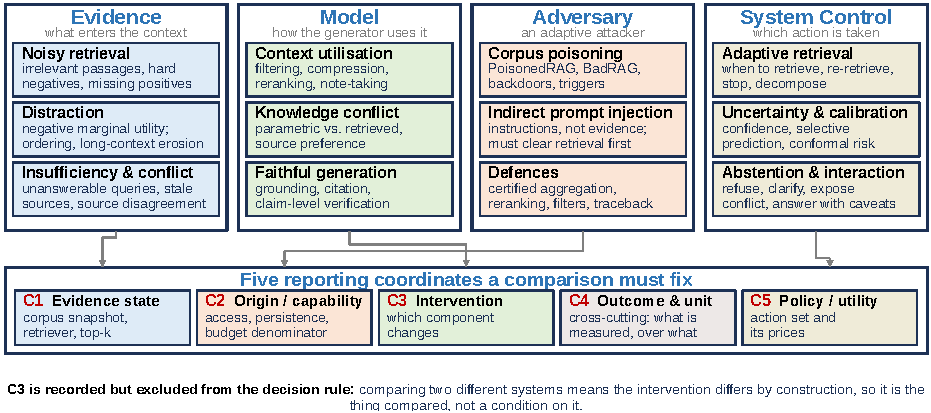
\includegraphics[width=\textwidth]{figures/generated/fig_taxonomy_map.pdf}%
\caption{The four failure surfaces and the reduction they support. Each column
is one surface of the survey (\S\ref{sec:evidence}--\S\ref{sec:system}); the
band below is the five reporting coordinates of \S\ref{sec:coordinates}, and the
connectors show which surface each coordinate collapses. C4 is cross-cutting
and has no single parent surface. The organisation is a partition of the
\emph{comparison} rather than of the literature: the columns tell a reader where
to look for related work, and the band tells a reader what must be stated on
both sides before two numbers can be placed together.}
\label{fig:hierarchical-taxonomy}
\end{figure*}

\begin{table*}[t]
\centering
\scriptsize
\renewcommand{\arraystretch}{0.88}
\begin{tabularx}{\linewidth}{>{\raggedright\arraybackslash}p{0.18\linewidth}>{\raggedright\arraybackslash}p{0.31\linewidth}>{\raggedright\arraybackslash}p{0.25\linewidth}X}
\toprule
\textbf{Boundary case} & \textbf{Rule used in this paper} & \textbf{Verdict consequence} & \textbf{Example implication} \\
\midrule
Noisy retrieval vs. distraction & Retrieval imperfection alone is coded as relevance/noise; harmful influence on generation, confidence, or reasoning is coded as distraction. & Same broad topic but different measured effect is partial. & Random negatives and hard distractors should not be pooled into one score. \\
Query/OOD vs. evidence state & Query ambiguity, distribution shift, and model uncertainty describe the need or belief state. Code them under origin unless the study labels the resulting retrieved evidence. & Shared uncertainty language does not imply a common evidence state or policy. & An OOD detector is not automatically an insufficient-context detector. \\
Natural conflict vs. adversarial corruption & Code by the source of contradiction, not by surface form. Naturally occurring or diagnostic contradiction is conflict; attacker-created contradiction is integrity/adversarial corruption. & Natural-conflict and poisoning results are invalid as a direct ranking unless the threat model is redefined. & Faithfulness or source-preference methods are not poisoning defenses by default. \\
Intervention mismatch & Code the component changed, then inspect the evaluation harness. Different interventions can be compared as alternatives if the remaining pipeline and target are controlled. & Shared harness and end-to-end target can support valid comparison; unmatched pipelines support only a qualified comparison. & A filter and a note-taking prompt can be compared after fixing retriever, generator, evidence states, budget, and action utility. \\
Metric overlap & Metric targets must match the object being measured. Accuracy, citation support, attack success, calibration, and selective risk are separate families. & Shared dataset but different metric family is partial; mutually incompatible targets are invalid for one-scalar ranking. & A correct answer with unsupported citation should not pass a faithfulness comparison. \\
Observable but unnamed action & Infer behavior only when action is decision-relevant and the protocol is unambiguous; otherwise use \emph{not applicable}. & Merely omitting the phrase ``action policy'' does not force under-specification. & An answer-only benchmark supplies \emph{answer} for a policy claim, but a fixed latency comparison needs no action label. \\
Security capability missing & Mark only decision-critical missing access, budget, objective, or target as unknown. A shared harness may intentionally vary capability. & Unknown capability makes a cross-game rank under-specified; controlled capability variation can support a valid descriptive contrast. & Black- and white-box variants of one attack can be compared inside the same harness without implying cross-paper transfer. \\
Benchmark vs. method & Code benchmark if the reusable artifact is the main contribution; otherwise code the intervention. & Benchmark-method comparison is partial unless the method is evaluated on the benchmark under aligned assumptions. & RGB is benchmark-first; RAAT is training-first. \\
Tuple match but control mismatch & After semantic coding, inspect corpus, data, retriever, generator, top-$k$, budget, baselines, decoding, and uncertainty. & A tuple match is insufficient for direct ranking when these factors confound the reported score. & Two answer-only noise methods on different datasets and generators require a shared rerun or a qualified claim. \\
\bottomrule
\end{tabularx}
\caption{Boundary rules for applying the revised diagnostic schema. Verdicts are claim-specific and require both semantic and experimental-control checks.}
\label{tab:taxonomy-rules}
\end{table*}

\begin{table*}[t]
\centering
\small
\begin{tabularx}{\linewidth}{p{0.14\linewidth}p{0.2\linewidth}p{0.27\linewidth}X}
\toprule
\textbf{Stage} & \textbf{Question} & \textbf{Typical signals} & \textbf{Representative actions} \\
\midrule
Detect & Is the current evidence unreliable? & Low retrieval confidence, high contradiction, low sufficient-context score, suspicious document patterns & Flag query/evidence, route to stronger checks, log risk state \\
Diagnose & What kind of unreliability is present? & Irrelevance, distraction, conflict, poisoning, ambiguity, unanswerability, stale evidence & Assign failure type; separate benign noise from adversarial risk \\
Mitigate & Can the evidence be repaired before answering? & Alternative retrieval results, filter scores, reranker utility, provenance, source agreement & Re-rank, filter, compress, re-query, retrieve from trusted sources, remove malicious passages \\
Control & What should the system do now? & Calibrated confidence, selective risk, cost budget, user risk tolerance & Answer, abstain, ask clarification, expose conflict, escalate to human review \\
Monitor & Did the system fail or get attacked? & User feedback, traceback signals, poisoned-document clusters, drift over time & Update index, quarantine sources, revise prompts, retrain filters, update audit logs \\
\bottomrule
\end{tabularx}
\caption{An operational pipeline for robust RAG. The pipeline turns the paper's taxonomy into actionable system design steps.}
\label{tab:operational-pipeline}
\end{table*}

\begin{figure*}[t]
\centering
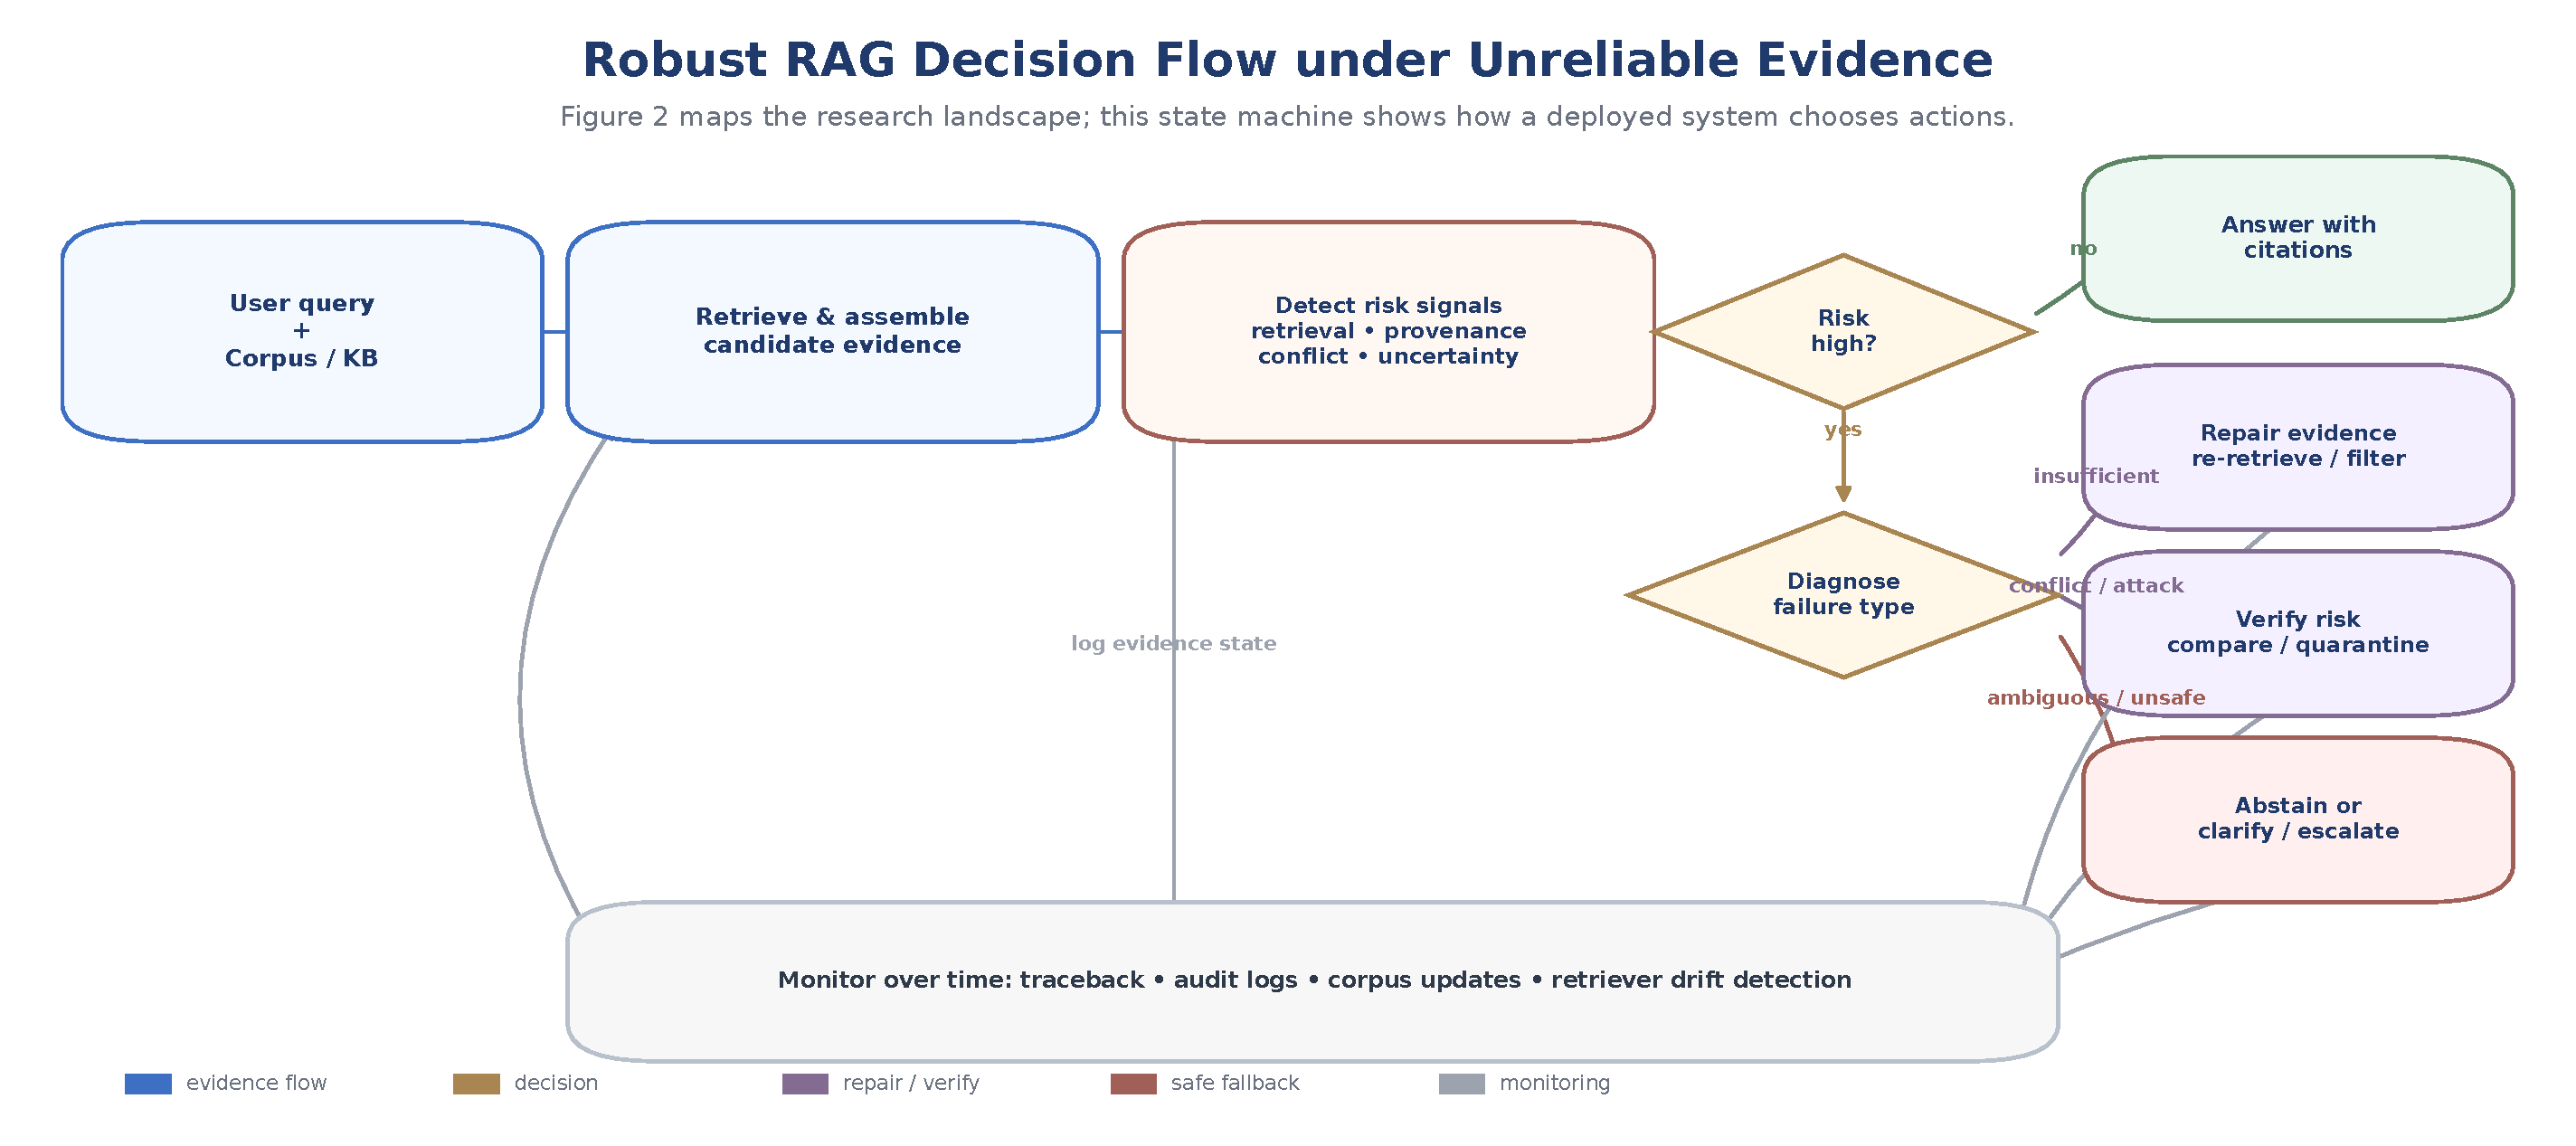
\includegraphics[width=\textwidth,keepaspectratio]{figures/generated/fig3_operational_decision_flow_py_4k.pdf}
\caption{Operational decision flow for robust RAG. Unlike the taxonomy in Figure~\ref{fig:hierarchical-taxonomy}, this state-machine view describes the branching actions a deployed system can take when unreliable evidence is encountered: answer, repair evidence, verify risk, abstain, clarify, escalate, or monitor.}
\label{fig:operational-pipeline-image}
\end{figure*}

\begin{table*}[t]
\centering
\small
\begin{tabularx}{\linewidth}{p{0.18\linewidth}p{0.18\linewidth}p{0.25\linewidth}X}
\toprule
\textbf{Theme} & \textbf{Representative work} & \textbf{Core idea} & \textbf{What it reveals for robust RAG} \\
\midrule
Irrelevant context & \citetalias{irrelevantContext2023} & Analyze and mitigate irrelevant retrieved context with filtering and robust training & Even answerable questions degrade when irrelevant passages enter the context; robustness is not equivalent to retrieval recall. \\
Retrieval-noise training & \citetalias{raat2024} & Categorize retrieval noise and train with adaptive adversarial objectives & Noise types should be separated: irrelevant, relevant-but-insufficient, and counterfactual evidence have different effects. \\
Generator note-taking & \citetalias{chainOfNote2023} & Generate per-passage notes before answering & Robust generation benefits from intermediate relevance judgments rather than direct answer generation. \\
Fine-grained noise benchmark & \citetalias{rrag027} & Configurable benchmark for distracting, low-quality, inconsequential, and irrelevant noise & ``Noise'' is not monolithic; evaluation should vary type, amount, and placement of bad evidence. \\
Nonlinear distraction & \citetalias{rrag003} & Study disproportionate effect of small amounts of misleading information & A few strong distractors can dominate long-context reasoning, so average noise rate is insufficient. \\
Long-context RAG & \citetalias{rrag039} & Analyze long-input RAG and hard negatives & More retrieved context can hurt unless ordering, filtering, or training adapts to long-context failure modes. \\
Sentence-level filtering & \citetalias{rrag044} & Filter retrieved context before generation & Filtering can be more fine-grained than document reranking and can remove local distractors inside otherwise useful passages. \\
Retrieval evaluation & \citetalias{rrag058} & Utility-aware retrieval metric for LLMs & RAG retrieval should be evaluated by downstream utility, including negative utility from distracting passages. \\
\bottomrule
\end{tabularx}
\caption{Representative evidence-centric work on noisy retrieval and distraction.}
\label{tab:evidence-methods}
\end{table*}

\begin{table*}[t]
\centering
\small
\begin{tabularx}{\linewidth}{p{0.2\linewidth}p{0.2\linewidth}p{0.28\linewidth}X}
\toprule
\textbf{Problem} & \textbf{Representative work} & \textbf{Mechanism} & \textbf{Limitation or open issue} \\
\midrule
Parametric--retrieved conflict & \citetalias{tugOfWar2024} & Construct and analyze conflicts between internal and external knowledge & Conflict behavior depends on model, prompt, evidence coherence, and task framing. \\
Fact-level conflict modeling & \citetalias{faithfulRAG2025} & Extract parametric self-facts, align them with retrieved facts, and reason before answering & Requires reliable fact extraction and alignment; complex claims remain difficult. \\
Source-aware consolidation & \citetalias{astuteRAG2025} & Elicit internal knowledge and consolidate it with retrieved sources using reliability comparison & Training-free but still depends on LLM self-assessment and source-quality cues. \\
Hidden-state rectification & \citetalias{rrag008} & Locate layers where parametric suppression occurs and contrast contextual/non-contextual logits & Promising for model-centric control, but model internals and transferability remain open. \\
Context utilisation benchmarks & \citetalias{rrag032} & Test gold, conflicting, and irrelevant contexts across models & Benchmarks reveal whether a model uses context, but not always why a model chooses one source. \\
Real-document conflict & \citetalias{rrag112} & Study behavior under context-memory conflicts with real documents & Realistic evidence can be messier than synthetic conflicts and harder to label. \\
Source preference & \citetalias{rrag132} & Analyze which sources win under conflict & Source preference may encode bias, recency effects, or authority priors. \\
\bottomrule
\end{tabularx}
\caption{Representative model-centric work on knowledge conflict and contextual faithfulness.}
\label{tab:conflict-methods}
\end{table*}

\begin{table*}[t]
\centering
\small
\begin{tabularx}{\linewidth}{p{0.17\linewidth}p{0.19\linewidth}p{0.25\linewidth}X}
\toprule
\textbf{Attack/defense surface} & \textbf{Representative work} & \textbf{Threat or defense} & \textbf{Implication} \\
\midrule
Retriever poisoning & \citetalias{poisoningRetrievalCorpora2023} & Inject adversarial passages to manipulate dense retrievers & Retrieval security can fail before generation begins. \\
RAG knowledge corruption & \citetalias{poisonedRAG2024} & Craft malicious passages that steer generated answers & End-to-end RAG needs corpus integrity and generation safeguards. \\
Backdoor attacks & \citetalias{trojanRAG2024}; \citetalias{phantom2024} & Triggered retrieval/generation behavior via poisoned contexts & RAG can act as a backdoor carrier without modifying model weights. \\
Prompt template attacks & \citetalias{aip2025} & Weaponize shared instructional prompts to steer retrieval and generation & Prompt templates are part of the attack surface, not just implementation details. \\
Indirect prompt injection & \citetalias{rrag005} & Optimize trigger fragments so malicious instructions are retrieved in the wild & Real attacks must overcome the retrieval barrier, not merely place malicious text in a corpus. \\
Certified defense & \citetalias{certifiedRAG2024} & Isolate-and-aggregate answers for robustness certificates & Certification gives stronger guarantees but typically assumes specific attack budgets. \\
Reranking defense & \citetalias{rrag004} & Use probe-gradient instability to demote poisoned passages & Defense can be inserted retriever-side without retraining the LLM. \\
Attention defense & \citetalias{rrag015} & Detect poisoning via normalised attention variance & Internal attention signals may expose poisoned evidence, but adaptivity remains a concern. \\
\bottomrule
\end{tabularx}
\caption{Representative adversarial corruption attacks and defenses.}
\label{tab:adversarial-methods}
\end{table*}

\begin{table*}[t]
\centering
\scriptsize
\renewcommand{\arraystretch}{0.88}
\begin{tabularx}{\linewidth}{>{\raggedright\arraybackslash}p{0.18\linewidth}c c c c >{\raggedright\arraybackslash}p{0.15\linewidth}X}
\toprule
\textbf{Threat class} & \textbf{Corpus} & \textbf{Query} & \textbf{Retr.} & \textbf{Gen.} & \textbf{Objective} & \textbf{Boundary} \\
\midrule
Dense-retriever poisoning \citep{poisoningRetrievalCorpora2023} & write & train set & white/gray & no & retrieve bad passages & Not always end-to-end. \\
RAG knowledge corruption \citep{poisonedRAG2024,badRAG2024} & write & target topic & black/gray & black & answer steering & Stealth/dynamics vary. \\
Backdoor-style RAG \citep{trojanRAG2024,phantom2024} & write & trigger & gray & black & latent behavior & Normal queries may pass. \\
Indirect prompt injection \citep{aip2025,rrag005} & write/share & natural & black & black & instruction hijack & Must overcome retrieval. \\
Opinion/fairness manipulation \citep{rrag104,rrag162} & write & group/topic & black/gray & black & bias steering & QA metrics miss social harm. \\
Defense setting \citep{certifiedRAG2024,rrag004,rrag015,rrag128} & bounded & varies & assumed & black/gray & detect/demote/trace & Depends on budget/visibility. \\
\bottomrule
\end{tabularx}
\caption{Attacker-capability matrix for adversarial RAG. The same ``attack success rate'' can mean different things depending on corpus write access, query control, retriever visibility, generator access, and objective.}
\label{tab:attacker-capability}
\end{table*}

\begin{table*}[t]
\centering
\scriptsize
\renewcommand{\arraystretch}{0.88}
\begin{tabularx}{\linewidth}{>{\raggedright\arraybackslash}p{0.17\linewidth}>{\raggedright\arraybackslash}p{0.21\linewidth}>{\raggedright\arraybackslash}p{0.22\linewidth}>{\raggedright\arraybackslash}p{0.16\linewidth}X}
\toprule
\textbf{Comparison} & \textbf{Why it looks comparable} & \textbf{Hidden mismatch} & \textbf{Metric pitfall} & \textbf{Normalised reading} \\
\midrule
PoisonedRAG vs. dense-retriever poisoning & Both insert malicious evidence into a retrieval corpus. & One evaluates end-to-end answer steering; the other may evaluate retriever ranking before generation. & Retrieval success and answer attack success are not the same target. & Compare only after recording whether poisoned evidence is retrieved and whether the generator changes the final answer. \\
Certified RAG defense vs. prompt-injection defense & Both are RAG defenses against corrupted retrieved content. & Certification assumes a bounded number of corrupted passages; prompt injection exploits instruction following rather than only false facts. & A certificate under bounded corruption may not imply instruction-hijack resistance. & Treat certification, instruction isolation, and document sanitisation as complementary defenses. \\
Traceback vs. prevention & Both reduce harm after poisoning. & Traceback identifies influential poisoned documents after failure; prevention attempts to block harmful output before response. & Lower post-hoc traceback error does not equal lower user-facing attack success. & Report prevention, detection, demotion, traceback, and recovery as separate outcome variables. \\
Backdoor trigger vs. natural query attack & Both can produce targeted malicious behavior. & Trigger attacks may rely on rare phrases; natural-query attacks must survive ordinary retrieval and ranking. & Attack success under attacker-crafted triggers overstates risk under natural user queries. & Require query-control and trigger-frequency fields before comparing attack strength. \\
\bottomrule
\end{tabularx}
\caption{Concrete examples of threat-model normalisation. These cases show how reported attack or defense success can reverse when attacker access, retrieval realism, and evaluation target differ.}
\label{tab:threat-model-examples}
\end{table*}


\begin{table*}[t]
\centering
\small
\begin{tabularx}{\linewidth}{p{0.16\linewidth}p{0.18\linewidth}p{0.28\linewidth}X}
\toprule
\textbf{Control/evaluation question} & \textbf{Representative work} & \textbf{Signal or decision} & \textbf{Why it matters} \\
\midrule
When to retrieve & \citetalias{selfRAG2023}; \citetalias{whenToRetrieve2024}; \citetalias{ctrla2025} & Reflection tokens, special retrieval tokens, or representation-based confidence/honesty directions & Retrieval is an action with costs and risks, not a fixed preprocessing step. \\
When retrieval is weak & \citetalias{crag2024}; \citetalias{sufficientContext2024} & Retrieval evaluator or sufficient-context signal & A system should repair or abstain rather than answer from insufficient evidence. \\
Calibration & \citetalias{calibRAG2025}; \citetalias{uncertaintyRAG2024}; \citetalias{rrag007} & Decision calibration, span uncertainty, verbal confidence calibration & Robustness requires confidence to reflect both model and evidence uncertainty. \\
Unanswerability & \citetalias{rrag111}; \citetalias{rrag141} & Unanswerable and underspecified RAG benchmarks & Real users often ask questions the corpus cannot answer; refusal and clarification need direct evaluation. \\
RAG capabilities & \citetalias{rgb2023} & Noise robustness, negative rejection, integration, counterfactual robustness & Multi-axis evaluation exposes failures hidden by answer accuracy. \\
Hallucination detection & \citetalias{ragTruth2024} & Word-level hallucination annotations for RAG outputs & Fine-grained labels support detection and attribution beyond answer-level scoring. \\
Query robustness & \citetalias{queryRobustness2025} & Perturb query wording and measure pipeline sensitivity & Robustness must include the query-to-retrieval interface. \\
\bottomrule
\end{tabularx}
\caption{Representative work on system-centric control and evaluation.}
\label{tab:control-eval-methods}
\end{table*}

\begin{table*}[t]
\centering
\scriptsize
\renewcommand{\arraystretch}{0.9}
\begin{tabularx}{\linewidth}{>{\raggedright\arraybackslash}p{0.18\linewidth}>{\raggedright\arraybackslash}p{0.22\linewidth}>{\raggedright\arraybackslash}p{0.25\linewidth}X}
\toprule
\textbf{Lineage} & \textbf{Classical question} & \textbf{RAG-specific version} & \textbf{Why it matters for robust RAG} \\
\midrule
Selective prediction & When should a model abstain to control risk? & Abstain when retrieved evidence is insufficient, conflicting, stale, or corrupted. & Selective risk must condition on evidence state, not only answer confidence. \\
Calibration & Does confidence match correctness? & Does confidence match answer correctness, evidence sufficiency, citation support, and retrieval usefulness? & A calibrated answer probability can still hide unreliable evidence. \\
Active clarification & When should the system ask a user for more information? & Ask clarification before retrieval when the query is ambiguous or underspecified. & Clarification can be the correct action even when retrieval could produce a plausible answer. \\
Cost-sensitive retrieval & When is additional computation worth it? & Decide whether to retrieve, re-retrieve, verify, rerank, or escalate under latency/cost budgets. & Robustness gains should be reported with action cost and coverage, not only accuracy. \\
Decision-theoretic control & Which action minimizes expected risk? & Choose among answer, abstain, expose conflict, cite uncertainty, retrieve again, or quarantine evidence. & Action quality is the bridge between evidence reliability estimates and user-facing behavior. \\
\bottomrule
\end{tabularx}
\caption{Action-control lineage. The framework imports ideas from selective prediction, calibration, clarification, and cost-sensitive decision-making, but makes retrieved evidence state the object being controlled.}
\label{tab:action-control-lineage}
\end{table*}



\section{Evaluation Details}
\label{sec:appendix-eval}
% Drawn by scripts/revision3/fig_appendix_schematics.py; the .pptx is the
% editable source and is released with the paper.
\begin{figure*}[t]
\centering
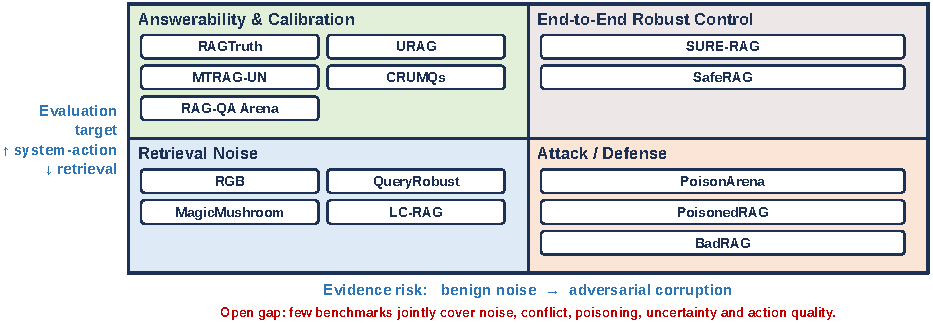
\includegraphics[width=\textwidth]{figures/generated/fig_benchmark_landscape.pdf}%
\caption{Conceptual benchmark landscape. Placement is illustrative rather than
data-derived; the figure organises differences in evidence risk and evaluation
level, not empirical distance or benchmark quality. The two axes are
coordinates C1 and C4, and the open gap is the reason a single ``robustness''
number rarely transfers between quadrants.}
\label{fig:benchmark-landscape}
\end{figure*}

\begin{table*}[t]
\centering
\scriptsize
\renewcommand{\arraystretch}{0.95}
\begin{tabularx}{\linewidth}{>{\raggedright\arraybackslash}p{0.12\linewidth}>{\raggedright\arraybackslash}p{0.13\linewidth}>{\raggedright\arraybackslash}p{0.17\linewidth}>{\raggedright\arraybackslash}p{0.18\linewidth}>{\raggedright\arraybackslash}p{0.14\linewidth}X}
\toprule
\textbf{Benchmark} & \textbf{Risk focus} & \textbf{Task / data} & \textbf{Perturbation or threat} & \textbf{Metrics} & \textbf{Boundary} \\
\midrule
RGB \citep{rgb2023} & noise, rejection, integration, counterfactuality & English/Chinese QA & noisy passages, false evidence, negative evidence & accuracy, ability-specific scores & Broad diagnostic benchmark but not adaptive attack-oriented. \\
RAGTruth \citep{ragTruth2024} & hallucination / faithfulness & QA, data-to-text, summarization & naturally generated unsupported spans & word-level hallucination labels & Strong annotation granularity; less focused on retrieval-side threat models. \\
Sufficient Context \citep{sufficientContext2024} & answerability & QA with context sufficiency labels & insufficient retrieved evidence & selective generation / abstention & Captures answerability but not adversarial corruption. \\
MagicMushroom \citep{rrag027} & retrieval noise & configurable RAG stress tests & distracting, low-quality, inconsequential, irrelevant noise & robustness under noise types & Fine-grained noise; limited conflict/security coverage. \\
URAG \citep{rrag001} & uncertainty & RAG as MCQA / conformal prediction & irrelevant/noisy retrieval and uncertainty sets & coverage, set size, calibration & Good for uncertainty; less direct for free-form generation. \\
QueryRobust \citep{queryRobustness2025} & query robustness & QA with query perturbations & wording variation at query--retrieval interface & retrieval and end-task degradation & Focuses on query perturbation, not corpus corruption. \\
PoisonArena \citep{rrag023} & adversarial poisoning & RAG attack competition setting & competing poisoning attacks & attack success, retrieval effects & Strong security focus; benign uncertainty is secondary. \\
SafeRAG \citep{rrag019} & RAG security & security benchmark for RAG & poisoning / malicious retrieval contexts & attack and defense metrics & Security-oriented; not a full evidence reliability suite. \\
MTRAG-UN \citep{rrag141} & multi-turn unanswerability & multi-turn RAG conversations & unanswerable, underspecified, non-standalone questions & abstention / clarification quality & Covers interaction; less focused on adversarial evidence. \\
CRUMQs \citep{rrag193} & unanswerable multi-hop RAG & realistic multi-hop queries & unanswerable and uncheatable questions & answerability and robustness & Useful for abstention; not a broad attack/noise benchmark. \\
\bottomrule
\end{tabularx}
\caption{Benchmark-level comparison for robust RAG evaluation. The table makes explicit what each benchmark perturbs, what it measures, and which failure modes remain outside its scope.}
\label{tab:benchmark-comparison}
\end{table*}


\begin{table*}[t]
\centering
\scriptsize
\begin{tabularx}{\linewidth}{p{0.18\linewidth}p{0.22\linewidth}p{0.24\linewidth}X}
\toprule
\textbf{Benchmark component} & \textbf{Required annotation} & \textbf{Metric suite} & \textbf{Why it is needed} \\
\midrule
Evidence reliability & relevance, sufficiency, freshness, provenance, support span & retrieval recall, sufficient-context accuracy, support precision & Distinguishes merely related passages from answer-supporting evidence. \\
Distraction and conflict & distractor type, conflicting claim pair, source agreement & answer flip rate, conflict sensitivity, context-utilisation score & Reveals whether models ignore harmful context or silently pick a source. \\
Adversarial corruption & attacker access, insertion budget, trigger type, poisoned document ID & attack success, poisoned retrieval rate, stealth, defense bypass & Makes security results comparable across threat models. \\
Unanswerability and ambiguity & answerability label, ambiguity type, clarification target & selective risk, abstention precision/recall, clarification accuracy & Evaluates robust action selection, not just answer generation. \\
Cost and system action & number of retrievals, verifier calls, latency, final action trace & cost-adjusted accuracy, action utility, coverage--risk curve & Prevents methods from hiding robustness gains behind unbounded computation. \\
\bottomrule
\end{tabularx}
\caption{A proposed benchmark blueprint for robust RAG under unreliable evidence. This is a research agenda rather than a validated leaderboard; existing benchmarks cover parts of the schema.}
\label{tab:benchmark-blueprint}
\end{table*}

\begin{table*}[t]
\centering
\scriptsize
\renewcommand{\arraystretch}{0.88}
\begin{tabularx}{\linewidth}{>{\raggedright\arraybackslash}p{0.16\linewidth}>{\raggedright\arraybackslash}p{0.20\linewidth}>{\raggedright\arraybackslash}p{0.20\linewidth}>{\raggedright\arraybackslash}p{0.18\linewidth}X}
\toprule
\textbf{Pilot item type} & \textbf{Evidence state label} & \textbf{Correct action trace} & \textbf{Answer metric alone would say} & \textbf{Action-aware diagnosis} \\
\midrule
Benign hard negative & Gold evidence present; hard negative ranked above it & retrieve $\rightarrow$ rerank/filter $\rightarrow$ answer with support & Correct/incorrect answer & Separates retriever ranking error from generator distraction. \\
Insufficient context & Retrieved context related but lacks answer-bearing span & retrieve $\rightarrow$ detect insufficiency $\rightarrow$ re-retrieve or abstain & Wrong answer or refusal & Rewards abstention/retrieval control rather than forced guessing. \\
Retrieved conflict & Two sources disagree with different dates/provenance & retrieve $\rightarrow$ compare sources $\rightarrow$ expose conflict or prefer fresher source & One answer may match gold & Checks whether the system hides unresolved conflict. \\
Poisoned evidence & Malicious document retrieved with plausible support & retrieve $\rightarrow$ detect/demote/quarantine $\rightarrow$ answer or abstain & Attack success/failure & Distinguishes poisoned retrieval, defense detection, and final answer steering. \\
\bottomrule
\end{tabularx}
\caption{Illustrative action-trace pilot for the benchmark blueprint. This is a worked annotation example, not a released leaderboard or empirical system ranking.}
\label{tab:action-trace-pilot}
\end{table*}


\begin{table}[t]
\centering
\small
\begin{tabular}{lrrr}
\toprule
\textbf{Toy policy} & \textbf{Ans.} & \textbf{Act.} & \textbf{Joint} \\
\midrule
Answer-only & 0.25 & 0.25 & 0.25 \\
Abstain-on-missing & 0.67 & 0.50 & 0.50 \\
Evidence-action oracle & 1.00 & 1.00 & 1.00 \\
\bottomrule
\end{tabular}
\caption{Action-trace pilot over 12 synthetic diagnostic items. Answer accuracy, action accuracy, and joint answer-action accuracy diagnose different behavior.}
\label{tab:action-trace-pilot-results}
\end{table}


\begin{table*}[t]
\centering
\scriptsize
\renewcommand{\arraystretch}{0.92}
\begin{tabularx}{\linewidth}{>{\raggedright\arraybackslash}p{0.17\linewidth}>{\raggedright\arraybackslash}p{0.27\linewidth}>{\raggedright\arraybackslash}p{0.25\linewidth}X}
\toprule
\textbf{Axis} & \textbf{Typical variation across papers} & \textbf{Why conclusions fail to transfer} & \textbf{Minimum reporting requirement} \\
\midrule
Retriever/generator setting & BM25 vs dense vs hybrid retrieval; small vs frontier generators; frozen vs fine-tuned models & A defense may work by compensating for one retriever or one model scale rather than solving the failure mode. & Retriever, index, top-$k$, reranker, generator, prompt, decoding, and context length. \\
Attack budget and access & Poisoned-document count, corpus write access, query control, retriever visibility, generator access & Attack success rates are incomparable when one attacker edits a corpus and another only controls the query. & Capability matrix, insertion budget, target set, stealth objective, and whether malicious evidence is retrieved. \\
Metric target & EM/F1, faithfulness, citation support, attack success, calibration error, selective risk, cost & Improving answer accuracy can worsen citation faithfulness; improving abstention can reduce coverage; reducing attacks can lower utility. & Report utility, evidence support, risk, calibration, cost, and security as a Pareto surface. \\
Statistical and reproducibility evidence & Single seed/model vs multiple seeds/models; code/data availability varies & Small prompt or model changes can reverse robustness rankings, especially for LLM-as-judge or attack benchmarks. & Seeds, confidence intervals or bootstrap tests where feasible, released prompts, data splits, and code or exact API settings. \\
Long-context baseline & RAG-only comparisons vs long-context LLMs with the same documents & A robustness gain may reflect retrieval compression rather than evidence reliability control. & Include a long-context or full-context baseline when context length permits, and report latency/cost. \\
Attribution vs answer accuracy & Some tasks score only final answer; others require evidence-supported citations & A model can answer correctly for the wrong reason, cite irrelevant evidence, or ignore retrieved support. & Claim-level support labels, citation precision/recall, and answer correctness reported separately. \\
\bottomrule
\end{tabularx}
\caption{Evaluation-assumption matrix for robust RAG. The table summarises why benchmark results often cannot be compared without aligning system setup, threat model, metric target, reproducibility evidence, and long-context baselines.}
\label{tab:evaluation-assumption-matrix}
\end{table*}


% Drawn by scripts/revision3/fig_appendix_schematics.py; the .pptx is the
% editable source and is released with the paper.
\begin{figure*}[t]
\centering
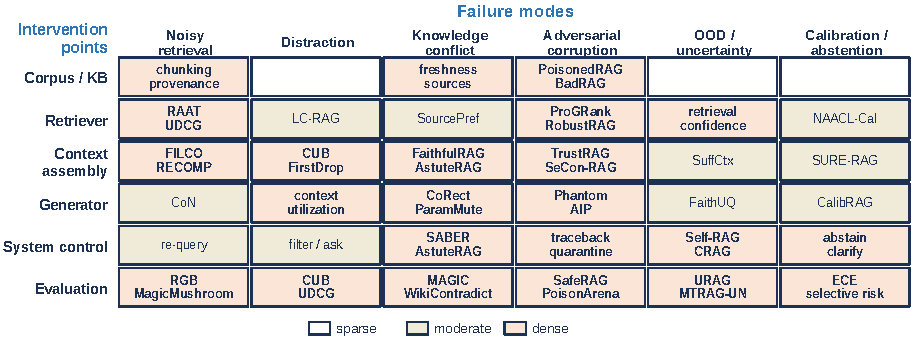
\includegraphics[width=\textwidth]{figures/generated/fig_failure_matrix.pdf}%
\caption{Schematic literature-family $\times$ intervention matrix. Shading and
example labels are illustrative design aids, not counts from Map~B;
quantitative Map-B distributions appear in Table~\ref{tab:corpus-stats}. Rows
are coordinate C3 and columns are coordinate C1, which is why a cell, not a
column, is the unit at which two systems become comparable.}
\label{fig:failure-intervention-matrix}
\end{figure*}

\begin{table*}[t]
\centering
\scriptsize
\renewcommand{\arraystretch}{0.92}
\begin{tabularx}{\linewidth}{>{\raggedright\arraybackslash}p{0.13\linewidth}>{\raggedright\arraybackslash}p{0.12\linewidth}>{\raggedright\arraybackslash}p{0.16\linewidth}>{\raggedright\arraybackslash}p{0.18\linewidth}>{\raggedright\arraybackslash}p{0.13\linewidth}>{\raggedright\arraybackslash}X}
\toprule
\textbf{Work} & \textbf{Failure} & \textbf{Task / setup} & \textbf{Key assumption} & \textbf{Metric} & \textbf{Boundary} \\
\midrule
IrrelCtx & irrelevant context & Open-domain QA & Irrelevance can be filtered or learned against & Robust accuracy & No adversarial/conflict setting. \\
RAAT & retrieval noise & Noisy QA training & Noise-aware training improves generation & F1/EM & Needs deployment-like noise. \\
RGB & multi-ability RAG & Bilingual benchmark & RAG reliability decomposes into abilities & Ability accuracy & Not adversarially adaptive. \\
FaithfulRAG & conflict & Fact-level conflict & Conflicts can be localised and reasoned over & Faithfulness & Needs reliable fact extraction. \\
AstuteRAG & imperfect retrieval & Training-free consolidation & Internal/external knowledge can be reliability-compared & Robust QA & Depends on LLM self-assessment. \\
PoisonedRAG & poisoning & Injected passages & Few crafted passages can dominate retrieval & Attack success & Targeted corruption focus. \\
RobustRAG & defense & Bounded corruption & Isolate-and-aggregate can certify robustness & Certificate, accuracy & Assumes attack budget. \\
Self-RAG / CtrlA & adaptive retrieval & Retrieve-or-answer & Model state can trigger retrieval & Trigger quality & Calibration can shift. \\
CalibRAG / URAG & calibration & Decision/MCQA & Confidence should reflect evidence uncertainty & ECE, coverage & Does not repair evidence. \\
PoisonArena / SafeRAG & security eval. & Poisoning benchmark & Threat models must be explicit & ASR, bypass & Still isolates attacks. \\
\bottomrule
\end{tabularx}
\caption{Analytical matrix of representative robust RAG work. Compared with a citation list, the matrix highlights each work's task setup, central assumption, metric focus, and boundary of applicability.}
\label{tab:analytical-matrix}
\end{table*}

\begin{table*}[t]
\centering
\scriptsize
\renewcommand{\arraystretch}{0.86}
\begin{tabularx}{\linewidth}{>{\raggedright\arraybackslash}p{0.13\linewidth}>{\raggedright\arraybackslash}p{0.17\linewidth}>{\raggedright\arraybackslash}p{0.17\linewidth}>{\raggedright\arraybackslash}p{0.16\linewidth}>{\raggedright\arraybackslash}p{0.13\linewidth}X}
\toprule
\textbf{Work} & \textbf{System setup} & \textbf{Failure construction} & \textbf{Metric / cost} & \textbf{Main claim} & \textbf{Failure boundary} \\
\midrule
IrrelCtx & RALM / open-domain QA; retrieved context injected into generator & Irrelevant passages with varying plausibility & Robust accuracy / answer degradation & Models can be brittle to irrelevant context. & Does not cover adversarial corruption or answerability policy. \\
RAAT & Noise-aware training for retrieval-augmented LMs & Multiple retrieval-noise types during training/evaluation & EM/F1 under noisy retrieval & Adaptive adversarial training improves noise robustness. & Transfer depends on whether deployment noise matches training noise. \\
RGB & Benchmark over English/Chinese QA-style RAG tasks & Noise, negative rejection, integration, counterfactual evidence & Ability-specific accuracy & RAG reliability decomposes into distinct abilities. & Benchmark abilities are diagnostic but not a unified control policy. \\
Sufficient Context & QA contexts labeled by sufficiency & Insufficient vs sufficient retrieved evidence & Selective answering / abstention quality & Evidence sufficiency should govern answerability. & Does not repair retrieval and does not model adversarial evidence. \\
PoisonedRAG & Corpus-injection attack against RAG & Crafted poisoned passages inserted into retrieval corpus & Attack success, retrieval of poison & Few poisoned documents can steer answers. & Strength depends on corpus write access, topic targeting, and retrieval success. \\
Certified / isolate defenses & Bounded-corruption RAG defense setting & Assumed corruption budget over retrieved evidence & Certificate, robust accuracy & Aggregation can certify robustness under budget assumptions. & Guarantees narrow when attacker violates budget or attacks instructions/tools. \\
Self-RAG / CtrlA & Adaptive retrieve-or-answer policies & Uncertainty about whether retrieval is needed & Trigger quality, answer utility, cost & Retrieval should be a conditional action. & Calibration shifts under distribution change; action cost often underreported. \\
RAGTruth & Annotated hallucination/faithfulness resource & Naturally generated unsupported spans across tasks & Span-level hallucination labels & Fine-grained support labels improve evaluation. & Faithfulness labels do not fully specify retrieval failure or system action. \\
\bottomrule
\end{tabularx}
\caption{Method-level comparison of representative robust-RAG work. The table makes explicit the setup, failure construction, metric target, main claim, and failure boundary that must be aligned before comparing methods.}
\label{tab:method-level-comparison}
\end{table*}


\begin{table*}[t]
\centering
\scriptsize
\renewcommand{\arraystretch}{0.86}
\begin{tabularx}{\linewidth}{>{\raggedright\arraybackslash}p{0.14\linewidth}>{\raggedright\arraybackslash}p{0.19\linewidth}>{\raggedright\arraybackslash}p{0.24\linewidth}>{\raggedright\arraybackslash}p{0.18\linewidth}X}
\toprule
\textbf{Case} & \textbf{Released rows / papers} & \textbf{Audited comparison fields} & \textbf{Metric or failure conflict} & \textbf{Synthesis / artifact boundary} \\
\midrule
Noise / distraction robustness & 5 rows: IrrelCtx, RAAT, Chain-of-Note, Sufficient Context, RGB & Assumption, QA dataset or benchmark slice, generator / reader setup, negative type, rank and gold-evidence availability. & EM/F1, rejection, selective risk, and ability-specific benchmark scores answer different questions. & Treat filtering, noise-aware training, generator reading, sufficiency prediction, and benchmark diagnosis as different mechanisms; artifact status is recorded per paper in the released worksheet. \\
Faithfulness, conflict, and attribution & 5 rows: RAGTruth, FaithfulRAG, AstuteRAG, Tug-of-War, Chain-of-Note & Unit of support, source-conflict assumption, attribution granularity, model-side reasoning setup, artifact availability. & Span-level support, fact-level conflict resolution, source preference, and final answer accuracy can disagree. & Citation faithfulness should not be collapsed into conflict robustness; the worksheet records where artifact evidence is dataset-level, code-level, or paper-only. \\
Adversarial corruption and RAG security & 6 rows: PoisonedRAG, corpus poisoning, BadRAG, certified defense, TrojanRAG, traceback & Corpus write access, insertion budget, retriever visibility, query control, generator access, stealth, retrieved malicious evidence, defense timing. & Attack success, certified robust accuracy, detection, traceback, and clean utility are not one defense score. & Compare only inside a capability envelope; prevention, demotion, detection, traceback, recovery, and certification remain separate outcomes. \\
Calibration, abstention, and adaptive control & 5 rows: Sufficient Context, Self-RAG, CRAG, CalibRAG, uncertainty RAG & Confidence target, evidence sufficiency labels, retrieval trigger, action set, cost budget, model/policy setup. & ECE, selective risk, coverage, retrieval-trigger quality, and answer utility can move in different directions. & Separate belief estimation from action selection; report coverage, cost, and final action alongside correctness. \\
Evaluation and benchmark comparability & 5 rows: RGB, RAGTruth, Sufficient Context, query robustness, RAG security benchmark & Evidence-state labels, perturbation source, model outputs scored, threat model, benchmark artifact availability. & Harder scores may reflect retrieval instability, unsupported spans, unanswerability, or adversarial steering. & Evaluation resources are diagnostic slices, not a universal robustness scale; benchmark comparisons require aligned evidence state and action policy. \\
\bottomrule
\end{tabularx}
\caption{Deeper case-study synthesis. The released 26-row worksheet compares assumptions, datasets or benchmark settings, model/evidence setup, metrics, failure modes, artifact availability, and comparison implications for the same five C1--C5 cases.}
\label{tab:deep-case-study-matrix}
\end{table*}

\begin{table*}[t]
\centering
\scriptsize
\renewcommand{\arraystretch}{0.9}
\begin{tabularx}{\linewidth}{>{\raggedright\arraybackslash}p{0.24\linewidth}>{\raggedright\arraybackslash}p{0.25\linewidth}>{\raggedright\arraybackslash}p{0.21\linewidth}X}
\toprule
\textbf{Main claim} & \textbf{Cited evidence basis} & \textbf{What the evidence supports} & \textbf{Boundary} \\
\midrule
Irrelevant or noisy context can harm generation. & Irrelevant-context robustness, RAAT, RGB, and counterfactual-noise studies. & Noise affects both retrieval quality and generator context use. & Does not imply one robustness score covers all noise types. \\
Knowledge conflict differs from adversarial corruption. & Conflict and poisoning studies with different evidence origins and evaluation targets. & Natural disagreement and attacker-created contradiction require different assumptions. & Conflict-resolution results should not be read as poisoning-defense results. \\
RAG attacks require capability normalisation. & Poisoning, backdoor, prompt-injection, traceback, and certification studies. & Attack/defense results require corpus access, query control, retriever visibility, and budget. & The paper does not rank attacks by real-world prevalence. \\
Calibration, abstention, and retrieval control are distinct. & Sufficient-context, uncertainty, adaptive-retrieval, and calibration studies. & Confidence estimation, evidence sufficiency, retrieval triggering, and abstention optimise different quantities. & Does not validate a single universal control policy. \\
Action-trace evaluation is a benchmark agenda. & Benchmarks exposing subsets of answer, evidence, action, cost, and threat fields. & Existing benchmarks cover pieces of the proposed schema. & No new leaderboard or empirical system ranking is claimed. \\
\bottomrule
\end{tabularx}
\caption{Narrative claim-to-source ledger. Expanded and strict citation audits
were model-assisted and deterministic; this table records the intended evidence
boundary rather than certifying every citation.}
\label{tab:claim-verification-ledger}
\end{table*}

\begin{table*}[t]
\centering
\scriptsize
\renewcommand{\arraystretch}{0.9}
\begin{tabularx}{\linewidth}{>{\raggedright\arraybackslash}p{0.15\linewidth}>{\raggedright\arraybackslash}p{0.24\linewidth}>{\raggedright\arraybackslash}p{0.27\linewidth}X}
\toprule
\textbf{Overlapping work} & \textbf{Typical interpretation in adjacent surveys} & \textbf{Reinterpretation under evidence reliability + action control} & \textbf{Different conclusion enabled} \\
\midrule
RGB / RAG evaluation benchmarks & A benchmark measuring multiple RAG abilities. & A diagnostic split between noisy evidence, negative rejection, integration, and counterfactual evidence states. & A single RAG score hides which system action failed: ignore, integrate, reject, or expose conflict. \\
Irrelevant-context robustness & A robustness method or context-filtering problem. & A generator-selectivity failure conditioned on retrieved but harmful context. & It should not be compared directly with retriever training unless the intervention point and context hardness are fixed. \\
Sufficient Context / answerability work & An abstention or uncertainty benchmark. & A control-policy problem: evidence sufficiency determines answer vs re-retrieve vs abstain. & Abstention accuracy is incomplete without evidence sufficiency and action-cost labels. \\
PoisonedRAG / RAG poisoning & A security attack surface. & An integrity failure whose strength depends on corpus write access, retrieval success, generator access, and insertion budget. & Attack success rates are not comparable until capability fields are normalized. \\
RAGTruth / hallucination evaluation & A faithfulness or hallucination annotation resource. & A separation between answer correctness, claim support, citation support, and evidence sufficiency. & Correct answers can still fail evidence reliability; citation faithfulness and answer accuracy should be reported separately. \\
Self-RAG / adaptive retrieval & A retrieval-augmented generation method. & A system-control policy that chooses retrieve, critique, answer, or continue under uncertainty. & The relevant evaluation target is not only answer quality but whether the policy chose the right action at the right cost. \\
\bottomrule
\end{tabularx}
\caption{How the same papers are interpreted differently under the proposed framework. This table grounds the novelty claim in concrete reinterpretations rather than broad positioning statements.}
\label{tab:overlap-reinterpretation}
\end{table*}



\section{Exploratory Map Statistics}
\label{sec:map-statistics}
\begin{table*}[t]
\centering
\small
\begin{tabularx}{\linewidth}{p{0.18\linewidth}X}
\toprule
\textbf{Dimension} & \textbf{Distribution in the 342-paper adjudicated Map B} \\
\midrule
Publication year & 2025: 170; 2024: 92; 2026: 65; 2023: 12; 2021: 2; 2022: 1 \\
Source / venue type & arXiv/preprint: 207; venue/proceedings-linked: 126; workshop/challenge: 5; other/unclear: 4 \\
Primary failure category & adversarial corruption: 120; knowledge conflict: 57; calibration/control: 55; evaluation/benchmark: 43; noisy retrieval: 34; distraction: 18; extension layer: 7; survey/background: 6; OOD/uncertainty: 2 \\
Method family & defense/mitigation: 119; attack: 75; benchmark/evaluation: 67; control/calibration: 27; method/evaluation: 21; analysis: 21; survey background: 6; conflict modeling: 4; method: 2 \\
Intervention point & generator: 81; corpus/KB: 67; evaluation: 51; context assembly: 48; mixed: 43; system control: 36; retriever/context: 15; not applicable: 1 \\
\bottomrule
\end{tabularx}
\caption{Descriptive corpus statistics for the canonical 342-row adjudicated Map B. These are map statistics, not field-wide prevalence estimates. Map A remains the IAA/adjudication snapshot.}
\label{tab:corpus-stats}
\end{table*}

\begin{table}[t]
\centering
\small
\begin{tabular}{lr}
\toprule
\textbf{Evidence stratum} & \textbf{Count} \\ 
\midrule
arXiv / preprint & 207 \\ 
venue / proceedings-linked & 126 \\ 
workshop / challenge & 5 \\ 
other / unclear & 4 \\ 
\bottomrule
\end{tabular}
\caption{Source strata in the canonical 342-row adjudicated Map B. Venue-linked coverage is now substantial relative to Map A, but the map remains a scoping corpus rather than a venue-complete census.}
\label{tab:evidence-strength}
\end{table}

\begin{table*}[t]
\centering
\scriptsize
\begin{tabular}{lrrrrrrrr}
\toprule
 & Noise & Distract & Conflict & Attack & OOD & Control & Eval. & Ext. \\ 
\midrule
Noise & 86 & 39 & 27 & 10 & 3 & 26 & 19 & 0 \\ 
Distract & 39 & 51 & 11 & 3 & 0 & 5 & 11 & 0 \\ 
Conflict & 27 & 11 & 104 & 22 & 5 & 20 & 34 & 1 \\ 
Attack & 10 & 3 & 22 & 135 & 1 & 10 & 21 & 0 \\ 
OOD & 3 & 0 & 5 & 1 & 40 & 34 & 10 & 0 \\ 
Control & 26 & 5 & 20 & 10 & 34 & 85 & 22 & 2 \\ 
Eval. & 19 & 11 & 34 & 21 & 10 & 22 & 90 & 1 \\ 
Ext. & 0 & 0 & 1 & 14 & 0 & 2 & 1 & 26 \\ 
\bottomrule
\end{tabular}
\caption{Category overlap in the 342-row adjudicated Map B. Extension-layer labels merge the historical \texttt{modality\_scenario} and \texttt{multimodal\_agentic\_code} names; counts are map diagnostics, not field prevalence.}
\label{tab:category-overlap}
\end{table*}

\begin{table*}[t]
\centering
\scriptsize
\begin{tabular}{lrrrrrrrr}
\toprule
\textbf{Method family} & Noise & Distract & Conflict & Attack & Control & Eval. & Ext. & Survey \\ 
\midrule
defense/mitigation & 27 & 12 & 33 & 37 & 9 & 0 & 1 & 0 \\ 
attack & 0 & 0 & 0 & 75 & 0 & 0 & 0 & 0 \\ 
benchmark/evaluation & 3 & 1 & 11 & 8 & 4 & 40 & 0 & 0 \\ 
control/calibration & 0 & 0 & 0 & 0 & 26 & 0 & 0 & 0 \\ 
method/evaluation & 3 & 1 & 1 & 0 & 8 & 2 & 6 & 0 \\ 
analysis & 1 & 4 & 8 & 0 & 6 & 1 & 0 & 0 \\ 
other/background & 0 & 0 & 4 & 0 & 2 & 0 & 0 & 6 \\ 
\bottomrule
\end{tabular}
\caption{Primary method-family by primary failure-type cross-tabulation over the 342-row adjudicated Map B. The table describes the map, not field-wide prevalence.}
\label{tab:method-failure-crosstab}
\end{table*}


\section{Detailed Audit Artifacts}
\label{sec:audit-artifacts}
\begin{table*}[t]
\centering
\small
\begin{tabularx}{\linewidth}{p{0.18\linewidth}p{0.16\linewidth}X}
\toprule
\textbf{Stage} & \textbf{Count} & \textbf{Rule} \\
\midrule
Initial retrieval & 1,904 records & Keyword search over arXiv, ACL Anthology, OpenReview, USENIX, AAAI/ACM landing pages where open versions were available, plus curated robust/trustworthy RAG paper lists; search cutoff 2026-06-03. \\
Open full-text corpus & 1,445 PDFs & Downloaded only open PDFs; removed failed downloads, inaccessible files, and non-PDF artifacts. \\
Deduplicated candidates & 1,399 papers & Deduplicated by normalised title and arXiv/proceedings identifiers; retained the most complete metadata record when preprint and proceedings versions overlapped. \\
Relevance screening & 536 included papers & Included papers that study RAG robustness, reliability, uncertainty, calibration, faithfulness, attack/defense, or evaluation under unreliable evidence; excluded application-only RAG papers. \\
Core pool & 112 papers & Papers directly shaping the taxonomy, threat/failure model, intervention mechanisms, or evaluation framework. \\
Core reading set & 100 papers & Core papers used as main narrative anchors; the remaining 12 core-pool papers stay in the broader scoping set. \\
Base scoping set & 300 papers & Core papers plus representative supporting work across all taxonomy branches before venue follow-up triage. \\
Venue-augmented scoping set & 326 papers & Base scoping set plus 26 venue-linked additions after follow-up triage. \\
Candidate evidence records & 274 papers & Base evidence map of 250 papers plus 24 venue-linked additions, double-coded and adjudicated. \\
Map A adjudicated seed & 268 papers & Candidate evidence records retained after final adjudication; used for IAA/adjudication provenance. \\
Map-B candidate expansion & 416 papers & Map A plus 148 source-blind human-citation-audit additions and 20 enriched original rows; used for second-coding review. \\
Map B adjudicated synthesis map & 342 papers & Map A plus 74 retained additions after second coding and final adjudication; frozen for current descriptive statistics. Post-freeze discoveries enter a recall log until a new version is coded. \\
\bottomrule
\end{tabularx}
\caption{Screening-flow summary. Search ends on 2026-06-03; coding and adjudication artifacts freeze on 2026-06-15. The supplement provides query strings, source counts, rules, exclusions, hashes, and a post-freeze recall log.}
\label{tab:review-protocol}
\end{table*}

\begin{table*}[t]
\centering
\scriptsize
\renewcommand{\arraystretch}{0.92}
\begin{tabularx}{\linewidth}{>{\raggedright\arraybackslash}p{0.17\linewidth}>{\raggedleft\arraybackslash}p{0.07\linewidth}>{\raggedright\arraybackslash}p{0.24\linewidth}X}
\toprule
\textbf{Set} & \textbf{N} & \textbf{Audit artifact} & \textbf{Selection rule and role} \\
\midrule
Retrieved records & 1,904 & \texttt{search\_protocol.json} & Initial keyword and curated-list retrieval before PDF availability, deduplication, or relevance screening. \\
Open full-text PDFs & 1,445 & \texttt{pdfs/} & Records with open PDFs available for full-text inspection; inaccessible or non-PDF artifacts removed. \\
Deduplicated candidates & 1,399 & \texttt{all\_reviewed\_deduped.csv} & Normalized-title and identifier deduplication; one record retained for preprint/proceedings overlaps. \\
Relevant included papers & 536 & \texttt{all\_reviewed\_deduped.csv} & Papers with decision \texttt{core} (112) or \texttt{include} (424); background-adjacent papers (289) and excluded papers (574) are tracked separately. \\
Core pool & 112 & \texttt{decision=core} in \texttt{all\_reviewed\_deduped.csv} & Papers judged central to taxonomy, threat/failure models, intervention mechanisms, or evaluation design. \\
Core reading set & 100 & \texttt{core100\_full.csv} & Main narrative anchors. The 12 core-pool papers not in this set remain in the base scoping set rather than being discarded. \\
Base scoping set & 300 & \texttt{survey300\_full.csv} & Core pool plus representative supporting work across failure categories, method families, and evaluation settings before venue follow-up triage. \\
Venue-augmented scoping set & 326 & \texttt{survey\_set\_venue\_audited.csv} & Base scoping set plus 26 venue-linked papers added after follow-up triage. \\
Base evidence map & 250 & \texttt{evidence\_map.csv} & Original structured map used before venue follow-up triage. \\
Candidate evidence records & 274 & round2 full adjudication CSV & Base map plus venue-linked additions, double-coded by humans and adjudicated. \\
Map A adjudicated seed & 268 & \texttt{evidence\_map\_adjudicated.csv} & Candidate evidence records with final \texttt{include\_in\_evidence\_map=1}; used for IAA/adjudication provenance. \\
Source-blind citation audit & 300 & \texttt{citation\_annotations.csv} & Source-blind human citation decisions over the venue and extension pools; distinct from the base scoping set. \\
Map-B candidate expansion & 416 & candidate expansion CSV & Map A plus 148 candidate additions supported by the source-blind citation audit and 20 enriched original rows; used for second coding. \\
Map B adjudicated synthesis map & 342 & adjudicated Map-B CSV & Map A plus 74 retained additions after second-coding adjudication; used for current synthesis statistics. \\
\bottomrule
\end{tabularx}
\caption{Corpus-set ledger. Exact memberships are released as CSV files for Map A, the 416-row candidate expansion, and the 342-row adjudicated Map B.}
\label{tab:set-selection-ledger}
\end{table*}

\begin{table*}[t]
\centering
\scriptsize
\renewcommand{\arraystretch}{0.94}
\begin{tabularx}{\linewidth}{>{\raggedright\arraybackslash}p{0.18\linewidth}>{\raggedright\arraybackslash}p{0.23\linewidth}>{\raggedright\arraybackslash}p{0.24\linewidth}X}
\toprule
\textbf{Artifact / claim source} & \textbf{Verification performed} & \textbf{What is coding- or metadata-assisted} & \textbf{How it is used in the paper} \\
\midrule
Main narrative claims and central citations & Author inspection of full paper text for papers used to support central claims, tables, and figures. & Initial prioritization and category suggestions were LLM-assisted. & Used for qualitative synthesis and case-study comparisons. \\
Core reading set & 100 papers curated from the 112-paper core pool after full-text relevance checks for narrative fit. & Core-pool creation used relevance scores and pre-labels as triage signals. & Used as the main reading backbone; not claimed to be a reproducible top-100 ranking without author judgment. \\
Map A, 268-paper adjudicated seed & Metadata and structured fields manually cleaned; venue-candidate triage completed; 274 candidate records independently double-coded and adjudicated into 268 included evidence-map papers. & Initial candidate discovery and pre-labeling were LLM-assisted, but final Map-A labels use human adjudication for coder disagreements. & Used for IAA/adjudication provenance, with the caveat that it is not the current synthesis denominator. \\
Map-B candidate expansion, 416 rows & Map A merged with source-blind human citation audit over the venue/extension pools; 148 new candidate rows added and 20 original rows enriched. & Candidate additions use human citation-audit decisions and deterministic field completion before second coding. & Used as the candidate pool for second coding, not as the final synthesis denominator. \\
Map B, 342-paper adjudicated synthesis map & Two coders independently second-coded all 148 additions; final adjudication retained 74 and excluded 74. & The retained additions use adjudicated labels; excluded boundary rows remain available in the release package. & Used for current source-stratified synthesis and venue sensitivity; still not a field census. \\
Human double-coding package & Two anonymized human sources independently coded all 274 candidate evidence records before discussion; round-2 agreement is strong across taxonomy, intervention, evidence-strength, relevance, core, and inclusion fields. & Disagreements were resolved in the final adjudication file. & Used to report pre-adjudication IAA and produce final adjudicated evidence-map labels. \\
Venue metadata pass and triage & ACL Anthology title/abstract scan plus DBLP/OpenAlex query logs, title matching, and follow-up triage decisions. & Discovery is metadata-based; inclusion/exclusion decisions are author triage rather than independent double coding. & Used to update venue-linked coverage and quantify remaining systematic-review limits. \\
\bottomrule
\end{tabularx}
\caption{Verification and annotation provenance. The table separates full-text author inspection, coding-assisted labels, metadata-derived venue candidates, and non-adjudicated consistency diagnostics.}
\label{tab:verification-provenance}
\end{table*}

\begin{table*}[t]
\centering
\scriptsize
\renewcommand{\arraystretch}{0.9}
\begin{tabularx}{\linewidth}{>{\raggedright\arraybackslash}p{0.19\linewidth}>{\raggedright\arraybackslash}p{0.25\linewidth}>{\raggedright\arraybackslash}p{0.24\linewidth}X}
\toprule
\textbf{Item} & \textbf{What was done} & \textbf{What was hidden from annotators} & \textbf{What we do not claim} \\
\midrule
Round-2 coders & Two anonymized coding-source records cover the same 274 candidate evidence records. & Machine pre-labels, prior evidence-map labels, previous adjudication logs, and the other source's labels. & The public package does not establish qualifications or personnel overlap; we claim file-level provenance, not independently verified expertise. \\
Training / codebook & Coders used the double-coding protocol and codebook defining scope, legacy literature-family tag, method family, intervention point, evidence strength, and inclusion fields. & Prior LLM rationales and model confidence scores. & We do not claim the codebook is final for all RAG subareas; adjudication notes can still motivate revisions. \\
Pre-adjudication separation & IAA was computed from separately completed CSV files before adjudication. & Post-discussion labels were not used for IAA. & This establishes workflow separation in the files, not personnel independence beyond the anonymized records. \\
Adjudication & A final adjudication file resolved 469 field-level disagreements and produced the 268-paper Map-A seed. & Source labels were preserved and not overwritten. & We do not apply Map-A IAA to the 148 later Map-B additions. \\
Source-blind citation audit & One source-blind citation-audit record set coded 300 papers from the venue/extension pools; 168 audited rows entered or enriched Map B after de-duplication and relevance checks. & Paper IDs were source-normalised and the audit did not use Map-A disagreement labels. & We do not claim 416-row double-coding, inter-annotator agreement, or independently verified annotator provenance for this batch. \\
\bottomrule
\end{tabularx}
\caption{Annotation transparency for the coding round. The table distinguishes file-auditable workflow separation from qualifications and personnel independence that the blind package does not establish.}
\label{tab:annotation-transparency}
\end{table*}

\begin{table*}[t]
\centering
\scriptsize
\begin{tabularx}{\linewidth}{p{0.24\linewidth}p{0.14\linewidth}p{0.14\linewidth}X}
\toprule
\textbf{Field} & \textbf{Agreement} & \textbf{$\kappa$ / score} & \textbf{Interpretation} \\
\midrule
Full-text checked & 100.0\% & 1.00 & Both sources marked every evidence-map paper as full-text checked. \\
In-scope screening & 99.6\% & 0.92 & Near-complete agreement; only one screening disagreement remains for adjudication. \\
Relevance level & -- & 0.80 & Linear-weighted agreement is strong for exclude/background/support/core priority. \\
Primary failure type & 97.1\% & 0.96 & Very strong human agreement on the main taxonomy category. \\
Method family & 89.4\% & 0.86 & Strong agreement on attack, benchmark, control, method, and analysis families. \\
Intervention point & 93.4\% & 0.92 & Very strong agreement on pipeline placement. \\
Evaluation type & 94.9\% & 0.93 & Very strong agreement on metric/evaluation family. \\
Evidence strength & 97.8\% & 0.95 & Very strong agreement on proceedings/preprint/review-platform strata. \\
Core-candidate decision & 91.6\% & 0.80 & Strong agreement on whether papers should shape the core narrative. \\
Include in evidence map & 99.3\% & 0.85 & Strong agreement on evidence-map inclusion. \\
Secondary labels & 79.2\% exact & 0.83 Jaccard & Multilabel agreement is strong enough to support overlap analysis after adjudication. \\
Reproducibility evidence & 10.6\% exact & 0.20 Jaccard & Weak free-text agreement; retained as adjudicated audit metadata, not used for primary comparison or trend claims. \\
\bottomrule
\end{tabularx}
\caption{Round-2 human-human agreement on 274 candidate evidence records before adjudication. Structured labels show strong agreement, while the free-text reproducibility field is weak and is treated only as adjudicated audit metadata. Two anonymized human annotation sources independently coded the same records; remaining disagreements were resolved to produce the 268-row Map-A adjudicated seed. These IAA values do not apply to the 148 later Map-B additions.}
\label{tab:iaa}
\end{table*}

\begin{table*}[t]
\centering
\scriptsize
\renewcommand{\arraystretch}{0.94}
\begin{tabularx}{\linewidth}{>{\raggedright\arraybackslash}p{0.22\linewidth}>{\raggedright\arraybackslash}p{0.24\linewidth}>{\raggedright\arraybackslash}p{0.20\linewidth}X}
\toprule
\textbf{Claim} & \textbf{Status under venue-linked / peer-reviewed evidence} & \textbf{What changes without preprints} & \textbf{Interpretation} \\
\midrule
Retrieved evidence can harm generation even when relevant evidence exists. & Holds: supported by venue-linked work on irrelevant/noisy context, noise-robust training, counterfactual noise, and imperfect retrieval. & The range of stress-test variants shrinks. & This is a stable mechanism-level claim. \\
RAG security results require attacker-capability normalisation. & Holds partially: venue-linked security work covers poisoning, traceback, membership inference, and backdoor-style corpus attacks. & Many fine-grained attack variants and defenses remain preprint-heavy. & The capability matrix is stable; detailed landscape counts are emerging trends. \\
Calibration, abstention, and retrieval control are distinct decisions. & Holds conceptually with venue-linked answerability, relevance-assessment, and calibration/control papers. & Specific method rankings and benchmark prevalence become sparse. & The conceptual separation remains; empirical prevalence is not settled. \\
The evidence map is attack- and benchmark-heavy. & Does not become a field-wide claim. & Under peer-reviewed-only evidence, the sample is much smaller and more evaluation-heavy. & Treat distributional cross-tabs as corpus diagnostics, not prevalence estimates. \\
Action-trace benchmark blueprint should score answer, evidence state, action, and cost. & Supported as a design synthesis, not validated as a benchmark standard. & The proposal becomes less empirical and more normative. & Keep as a research agenda unless a full benchmark is built and evaluated. \\
\bottomrule
\end{tabularx}
\caption{Peer-reviewed / venue-linked sensitivity analysis. The table states which conclusions survive when preprint-only evidence is downweighted and which remain hypothesis-generating.}
\label{tab:peer-reviewed-sensitivity}
\end{table*}


\begin{table*}[t]
\centering
\scriptsize
\renewcommand{\arraystretch}{0.94}
\begin{tabularx}{\linewidth}{>{\raggedright\arraybackslash}p{0.20\linewidth}>{\raggedright\arraybackslash}p{0.25\linewidth}>{\raggedright\arraybackslash}p{0.18\linewidth}X}
\toprule
\textbf{Pass} & \textbf{Scope} & \textbf{Observed yield} & \textbf{Interpretation} \\
\midrule
ACL Anthology metadata scan & ACL, EMNLP, NAACL, COLING; 2020--2026; full anthology BibTeX with abstracts & 12,924 entries scanned; 181 RAG candidates; 30 robust-RAG candidates & A reproducible proceedings-level metadata scan for core NLP venues, not just backfilled metadata. \\
DBLP/OpenAlex metadata queries & 15 robust-RAG query strings over venue-linked metadata for SIGIR, WWW, WSDM, KDD, USENIX Security, CCS, NDSS, ICLR, NeurIPS and overlaps & 31 query rows; 51 unique venue-linked candidate titles after deduplication & Surfaced missing venue-linked candidates; all 51 were subsequently triaged. \\
Follow-up venue triage & 51 venue-linked candidates & 23 new evidence-map additions; 3 background additions; 9 exclusions; 2 duplicates; 13 already represented & Closes the unprocessed venue-candidate gap, while still not claiming complete manual proceedings coverage. \\
Map A adjudicated seed & 268 evidence-map papers & 42 venue/proceedings-linked; 222 arXiv-only or emerging preprints; 4 other strata & IAA/adjudication basis before venue expansion. \\
Map-B candidate expansion & 416 evidence-map candidates & 194 venue/proceedings-linked; 207 arXiv/preprint; 11 workshop/challenge; 4 other/unclear & Pre-adjudication candidate map after source-blind citation audit. \\
Map B adjudicated synthesis map & 342 evidence-map papers & 126 venue/proceedings-linked; 207 arXiv/preprint; 5 workshop/challenge; 4 other/unclear & Current source-stratified synthesis map after second coding and final adjudication. \\
\bottomrule
\end{tabularx}
\caption{Venue-oriented search, coverage audit, and follow-up triage summary. Full query logs, candidate titles, decisions, and limitations are in \texttt{venue\_systematic\_queries.csv}, \texttt{venue\_systematic\_candidates.csv}, \texttt{venue\_coverage\_audit.csv}, and \texttt{venue\_triage\_decisions.csv}.}
\label{tab:venue-pass-summary}
\end{table*}

\begin{table*}[t]
\centering
\scriptsize
\renewcommand{\arraystretch}{0.94}
\begin{tabularx}{\linewidth}{>{\raggedright\arraybackslash}p{0.20\linewidth}>{\raggedright\arraybackslash}p{0.18\linewidth}>{\raggedright\arraybackslash}p{0.18\linewidth}X}
\toprule
\textbf{Coverage check} & \textbf{Count} & \textbf{Artifact} & \textbf{Interpretation} \\
\midrule
Venue-linked robust-RAG candidates found by metadata pass & 51 unique titles & candidate CSV & Candidate pool from ACL Anthology, DBLP, and OpenAlex metadata queries. \\
Already in core100 & 6 / 51 & coverage audit CSV & Core narrative captures only a small subset of venue-linked candidates. \\
Already in base scoping set & 14 / 51 & coverage audit CSV & The current scoping set misses or intentionally excludes many venue-linked candidates. \\
Already in evidence map & 13 / 51 & coverage audit CSV & Cross-tabs should be interpreted as map statistics, not field statistics. \\
Not in original base scoping set & 37 / 51 & coverage audit CSV & These papers were subsequently triaged; see Table~\ref{tab:venue-triage-summary}. \\
\bottomrule
\end{tabularx}
\caption{Venue-coverage audit after the metadata pass. The audit quantifies residual coverage risk by matching venue-linked candidates against the original core, survey, and evidence-map sets. Files: \texttt{venue\_systematic\_candidates.csv} and \texttt{venue\_coverage\_audit.csv}.}
\label{tab:venue-coverage-audit}
\end{table*}

\begin{table*}[t]
\centering
\scriptsize
\renewcommand{\arraystretch}{0.9}
\begin{tabularx}{\linewidth}{>{\raggedright\arraybackslash}p{0.20\linewidth}>{\raggedright\arraybackslash}p{0.24\linewidth}>{\raggedright\arraybackslash}p{0.20\linewidth}X}
\toprule
\textbf{Recall check} & \textbf{Observed result} & \textbf{What it controls} & \textbf{Residual risk} \\
\midrule
ACL Anthology metadata scan & 12,924 entries scanned for ACL/EMNLP/NAACL/COLING; 181 RAG candidates; 30 robust-RAG candidates & Reduces reliance on arXiv-only discovery for core NLP venues. & Title/abstract terms can miss papers using older QA/IR terminology. \\
Cross-venue metadata pass & DBLP/OpenAlex queries yielded 51 venue-linked robust-RAG candidates & Adds IR, web, security, and ML venue-linked records. & API ranking, metadata naming, and transient query errors limit recall. \\
Follow-up triage & 51 candidates triaged; 26 added to scoping set; 24 added to evidence map; 9 excluded; 2 duplicates & Closes the known unprocessed venue-candidate gap. & Does not prove complete coverage of every proceedings volume. \\
Evidence-strength sensitivity & Main conclusions separated into venue-linked backbone vs preprint trend evidence & Prevents preprint-heavy map statistics from becoming field-level claims. & Some emerging security/control subtopics remain too new for strong consensus. \\
\bottomrule
\end{tabularx}
\caption{Venue-recall risk analysis. The venue pass improves auditability and adds missed venue-linked papers, but it is still not a manual venue-complete proceedings review.}
\label{tab:venue-recall-risk}
\end{table*}


\begin{table*}[t]
\centering
\scriptsize
\renewcommand{\arraystretch}{0.94}
\begin{tabularx}{\linewidth}{>{\raggedright\arraybackslash}p{0.22\linewidth}>{\raggedright\arraybackslash}p{0.15\linewidth}>{\raggedright\arraybackslash}p{0.20\linewidth}X}
\toprule
\textbf{Triage outcome} & \textbf{Count} & \textbf{Action} & \textbf{Reasoning} \\
\midrule
Already represented in base evidence map & 13 & retain & Candidate was already included; metadata pass only improved venue visibility. \\
New evidence-map additions & 23 & add to evidence extension & Directly studies robust RAG, RAG evaluation, evidence reliability, security, calibration, or robust generation. \\
Scoping-set paper promoted to evidence extension & 1 & add to evidence extension & Already in the scoping set but not the base map; venue audit identified it as relevant to trust/calibration. \\
Background additions & 3 & add to venue-augmented scoping set only & Relevant boundary papers on domain, multilingual, or multimodal RAG, but not central text evidence-reliability evidence. \\
Excluded false positives / applications & 9 & exclude with reason & Application or adjacent RAG papers without robustness/evidence-reliability analysis. \\
Duplicate venue records & 2 & deduplicate & Same work already represented through another metadata record. \\
\midrule
\textbf{Venue-augmented scoping set} & \textbf{326} & base 300 + 26 additions & Updated scoping set after follow-up triage. \\
\textbf{Map A adjudicated seed} & \textbf{268} & 274 candidates - 6 exclusions & IAA/adjudication snapshot after human adjudication of double-coded candidate evidence records. \\
\textbf{Map-B candidate expansion} & \textbf{416} & Map A + 148 citation-audit-supported additions & Pre-adjudication candidate map after source-blind citation audit. \\
\textbf{Map B adjudicated synthesis map} & \textbf{342} & Map A + 74 retained additions & Current evidence map for synthesis after second coding and adjudication. \\
\bottomrule
\end{tabularx}
\caption{Follow-up triage of all 51 venue-linked candidates from the metadata pass. The 37 candidates outside the original scoping set are no longer unprocessed; decisions and reasons are in \texttt{venue\_triage\_decisions.csv}.}
\label{tab:venue-triage-summary}
\end{table*}

\begin{table*}[t]
\centering
\scriptsize
\begin{tabularx}{\linewidth}{p{0.18\linewidth}p{0.42\linewidth}X}
\toprule
\textbf{Category} & \textbf{Definition} & \textbf{Inclusion rule} \\
\midrule
Noisy retrieval & Benign retrieval imperfection: irrelevant passages, hard negatives, missing positives, stale or low-quality evidence. & Explicitly analyzes or mitigates retrieval noise, not merely uses retrieval. \\
Distraction & Retrieved context has negative marginal utility and changes answer, confidence, or reasoning despite not supporting the answer. & Includes distractor, context-utilization, or long-context degradation analysis. \\
Knowledge conflict & Contradiction between parametric knowledge and retrieved evidence, or among retrieved sources. & Includes conflict detection, source preference, fact-level reconciliation, or contextual faithfulness. \\
Adversarial corruption & Adaptive attacker manipulates corpus, retriever, prompt template, retrieved context, memory, or tools. & Includes poisoning, prompt injection, backdoors, attack/defense benchmarks. \\
OOD / uncertainty & Query or evidence is ambiguous, underspecified, unanswerable, out-of-knowledge-base, or under distribution shift. & Includes answerability, uncertainty quantification, or selective prediction. \\
Calibration / control & System decides when to retrieve, trust evidence, answer, abstain, clarify, or escalate. & Includes adaptive retrieval, calibrated decision-making, or abstention. \\
Evaluation benchmark & Paper introduces benchmark, dataset, metric, or evaluation protocol for robust RAG. & Must define evaluation axis, data, perturbation/threat, or metric. \\
\bottomrule
\end{tabularx}
\caption{Taxonomy codebook used for paper categorization. The full codebook is provided in the supplementary material.}
\label{tab:codebook}
\end{table*}


\section{Core and Evidence Map Samples}
\begin{table*}[t]
\centering
\scriptsize
\begin{tabularx}{\linewidth}{p{0.05\linewidth}X p{0.24\linewidth} p{0.10\linewidth}}
\toprule
Rank & Paper & Categories & Role \\
\midrule
1 & PoisonedRAG: Knowledge Corruption Attacks to Retrieval-Augmented Generation of Large Language Models & adv. corruption & attack \\
2 & Certifiably Robust RAG against Retrieval Corruption & adv. corruption & defense \\
3 & Making Retrieval-Augmented Language Models Robust to Irrelevant Context & noisy retrieval; distraction; calibration & method \\
4 & Enhancing Noise Robustness of Retrieval-Augmented Language Models with Adaptive Adversarial Training & noisy retrieval; evaluation & defense \\
5 & Phantom: General Backdoor Attacks on Retrieval Augmented Language Generation & adv. corruption & attack \\
6 & URAG: A Benchmark for Uncertainty Quantification in Retrieval-Augmented Large Language Models & OOD/uncertainty; calibration; evaluation; noise & benchmark \\
7 & Trust or Abstain? A Self-Aware RAG Approach & knowledge conflict; calibration; evaluation & method \\
8 & The First Drop of Ink: Nonlinear Impact of Misleading Information in Long-Context Reasoning & distraction; noisy retrieval & analysis \\
\bottomrule
\end{tabularx}
\caption{Sample entries from the core reading set. The full core set and metadata are provided in the supplementary material.}
\label{tab:core-sample}
\end{table*}

\label{sec:lit-map}
\begin{table*}[t]
\centering
\scriptsize
\renewcommand{\arraystretch}{0.92}
\begin{tabularx}{\linewidth}{p{0.13\linewidth}p{0.12\linewidth}p{0.16\linewidth}p{0.15\linewidth}p{0.16\linewidth}X}
\toprule
\textbf{Paper} & \textbf{Year} & \textbf{Failure / risk} & \textbf{Method family} & \textbf{Intervention} & \textbf{Boundary / note} \\
\midrule
PoisonedRAG & 2025 & adversarial corruption & attack & corpus / KB & Targeted knowledge corruption; stealth and long-term dynamics vary. \\
RobustRAG & 2024 & adversarial corruption & defense & retriever / aggregation & Certification assumes bounded corruption. \\
IrrelCtx & 2023 & retrieval noise / distraction & defense & context filtering & Does not model adaptive attackers. \\
RAAT & 2024 & retrieval noise & training & generator & Requires deployment-like noisy training data. \\
FaithfulRAG & 2025 & knowledge conflict & conflict modeling & generator & Depends on fact extraction and alignment. \\
AstuteRAG & 2025 & imperfect retrieval + conflict & control / consolidation & system control & Relies on source-aware LLM self-assessment. \\
Self-RAG & 2024 & retrieval need & adaptive retrieval & system control & Retrieval trigger calibration can shift. \\
RGB & 2024 & multi-axis RAG failure & benchmark & evaluation & Not adversarially adaptive. \\
RAGTruth & 2024 & hallucination / faithfulness & benchmark & evaluation & Strong word-level labels, less retrieval-threat focus. \\
MTRAG-UN & 2026 & unanswerability & benchmark & system action & Multi-turn setting; security is secondary. \\
\bottomrule
\end{tabularx}
\caption{Sample of the structured evidence map. The full CSV supplement contains title, authors, year, source, taxonomy categories, failure/risk type, method family, intervention point, benchmark/task, metrics, contribution, and limitation/note for the cited literature map.}
\label{tab:evidence-map-sample}
\end{table*}



\end{document}
